\documentclass[10pt]{article}
\usepackage[margin=1in]{geometry}
\usepackage[all]{xy}

\usepackage[english]{babel}

\usepackage[nottoc]{tocbibind}

\usepackage{amsmath,amsthm,amssymb,color,latexsym}
\usepackage{geometry}        
\geometry{letterpaper}    
\usepackage{graphicx}
\usepackage{physics}

\usepackage{listings}
\usepackage[table,xcdraw]{xcolor}

\usepackage[export]{adjustbox}

\definecolor{codegreen}{rgb}{0,0.6,0}
\definecolor{codegray}{rgb}{0.5,0.5,0.5}
\definecolor{codepurple}{rgb}{0.58,0,0.82}
\definecolor{backcolour}{rgb}{0.95,0.95,0.92}
\usepackage{multirow}
\usepackage{float}

\lstdefinestyle{mystyle}{
  backgroundcolor=\color{backcolour},   commentstyle=\color{codegreen},
  keywordstyle=\color{magenta},
  numberstyle=\tiny\color{codegray},
  stringstyle=\color{codepurple},
  basicstyle=\ttfamily\footnotesize,
  breakatwhitespace=false,         
  breaklines=true,                 
  captionpos=b,                    
  keepspaces=true,                 
  numbers=left,                    
  numbersep=5pt,                  
  showspaces=false,                
  showstringspaces=false,
  showtabs=false,                  
  tabsize=2
}

\lstset{style=mystyle}

\usepackage{graphicx}
\graphicspath{ {./images/} }


\newtheorem{problem}{Problem}

\newenvironment{solution}[1][\it{Solution}]{\textbf{#1. } }{$\square$}


\begin{document}
\noindent CS 6140: Machine Learning Spring 2021\hfill Homework Assignment \#4\\
Sakshi Suman\hfill suman.sak@northeastern.edu

\hrulefill


\begin{problem}

Consider a logistic regression problem where $\mathcal{X}=\mathbb{R}^{d}$ and $\mathcal{Y}=\{-1,+1\}$. Derive the weight update rule that maximizes the conditional likelihood assuming that a data set $\mathcal{D}=\left\{\left(x_{i}, y_{i}\right)\right\}_{i=1}^{n}$ is given.

\end{problem}
\begin{solution}

To frame the learning problem as parameter estimation, let the data set $\mathcal{D}=\left\{\left(\mathbf{x}_{i}, y_{i}\right)\right\}_{i=1}^{n}$ is an i.i.d. sample from a fixed but unknown probability distribution $p(\mathbf{x}, y) .$ Even more specifically, we can assume that the data generating process randomly draws a data point $\mathrm{x},$ a realization of the random vector $\left(X_{0}=1, X_{1}, \ldots, X_{d}\right),$ according to $p(\mathbf{x})$ and then sets its class label $Y$ according to the Bernoulli distribution

\begin{equation*}
\scalebox{1.4}{
$p(y \mid \mathbf{x}) = 
        \begin{cases}
            \left(\frac{1}{1+e^{-\omega^{\top} \mathbf{x}}}\right)^{\frac{1+y}{2}} &\text{ for } y=1 \\
			  \left(1-\frac{1}{1+e^{-\omega^{\top} \mathbf{x}}}\right)^{\frac{1-y}{2}} &\text{ for } y=-1
        \end{cases}$
        }
    \end{equation*}

where $\omega=\left(\omega_{0}, \omega_{1}, \ldots, \omega_{d}\right)$ is a set of unknown coefficients we want to recover (or learn) from the observed data $\mathcal{D}$. Based on the principles of parameter estimation, we can estimate $\omega$ by maximizing the conditional likelihood of the observed class labels $\mathbf{y}=\left(y_{1}, y_{2}, \ldots, y_{n}\right)$ given the inputs $\mathbf{X}=\left(\mathbf{x}_{1}^{\top}, \mathbf{x}_{2}^{\top}, \ldots, \mathbf{x}_{n}^{\top}\right)$
We shall first write the conditional likelihood function $p(\mathbf{y} \mid \mathbf{X}, \mathbf{w}),$ or simply $l(\mathbf{w}),$ as
$$
l(\mathbf{w})=\prod_{i=1}^{n} p\left(y_{i} \mid \mathbf{x}_{i}, \mathbf{w}\right)
$$

The parameter vector that maximizes the likelihood is,

$$
\begin{aligned}
\mathbf{w}_{\mathrm{ML}} &=\underset{\mathbf{w}}{\arg \max }\{l(\mathbf{w})\} \\
&=\underset{\mathbf{w}}{\arg \max }\left\{\prod_{i=1}^{n} p\left(y_{i} \mid \mathbf{x}_{i}, \mathbf{w}\right)\right\} .
\end{aligned}
$$

The likelihood function is
$$
l(\mathbf{w})=\prod_{i=1}^{n}\left(\frac{1}{1+e^{-\mathbf{w}^{\top} \mathbf{x}_{i}}}\right)^{\frac{1+y_{i}}{2}} \cdot\left(1-\frac{1}{1+e^{-\mathbf{w}^{\top} \mathbf{x}_{i}}}\right)^{\frac{1-y_{i}}{2}}
$$

As $\log(x)$ is a strictly increasing function, maximizing likelihood is equivalent to maximizing the log-likelihood function $l l(\mathbf{w})=\log (l(\mathbf{w}))$
$$
l l(\mathbf{w})=\sum_{i=1}^{n}\left(\left(\frac{1+y_{i}}{2}\right) \cdot \log \left(\frac{1}{1+e^{-\mathbf{w}^{\top} \mathbf{x}_{i}}}\right)+\left(\frac{1-y_{i}}{2}\right) \cdot \log \left(1-\frac{1}{1+e^{-\mathbf{w}^{\top} \mathbf{x}_{i}}}\right)\right)
$$

The negative of the log-likelihood i.e., cross-entropy minimization is equivalent to the maximization of likelihood.

$$
ll(\mathbf{w})=\sum_{i=1}^{n}\left(\left(\frac{y_{i}-1}{2}\right) \mathbf{w}^{\top} \mathbf{x}_{i}+\log \left(\frac{1}{1+e^{-\mathbf{w}^{\top} \mathbf{x}_{i}}}\right)\right)
$$

There is no closed-form solution to $\nabla ll(\mathbf{w})=\mathbf{0}$. Thus, we have to proceed with iterative optimization methods. Hence the goal is to calculate the gradient $(\nabla ll(\mathbf{w}))$ and Hessian $\left(H_{l l(\mathbf{w})}\right)$ in order to specify the update rule described by Newton-Raphson's method, as a function of inputs $\mathbf{X}$, class labels $\mathbf{y},$ and the current parameter vector. We can calculate the first and second partial derivatives of $ll(\mathbf{w})$ as follows

$$
\begin{aligned}
\frac{\partial ll(\mathbf{w})}{\partial w_{j}} &=\sum_{i=1}^{n}\left(\left(\frac{y_{i}-1}{2}\right) \cdot x_{i j}-\frac{1}{1+e^{-\mathbf{w}^{\top} \mathbf{x}_{i}}} \cdot e^{-\mathbf{w}^{\top} \mathbf{x}_{i}} \cdot\left(-x_{i j}\right)\right) \\
&=\sum_{i=1}^{n} x_{i j} \cdot\left(\left(\frac{y_{i}-1}{2}\right)+\frac{e^{-\mathbf{w}^{\top} \mathbf{x}_{i}}}{1+e^{-\mathbf{w}^{\top} \mathbf{x}_{i}}}\right) \\
&=\sum_{i=1}^{n} x_{i j} \cdot\left(\left(\frac{y_{i} + 1}{2}\right)-\frac{1}{1+e^{-\mathbf{w}^{\top} \mathbf{x}_{i}}}\right) \\
&=\mathbf{f}_{j}^{\top}\left(\left(\frac{\mathbf{y}+\mathbf{1}}{2}\right)-\mathbf{p}\right)
\end{aligned}
$$

where $\mathbf{f}_{j}$ is the $j$ -th column (feature) of data matrix $\mathbf{X}, \mathbf{y}$ is an $n$-dimensional column vector of class labels, $\mathbf{1}$ is a vector containing $n$ 1s and $\mathbf{p}$ is an $n$-dimensional column vector of (estimated) posterior probabilities $p_{i}=P\left(Y_{i}=1 \mid \mathbf{x}_{i}, \mathbf{w}\right),$ for $i=1, \ldots, n$. Considering partial derivatives for every component of $\mathbf{w}$, we have
$$
\nabla ll(\mathbf{w})=\mathbf{X}^{T}\left(\left(\frac{\mathbf{y} + \mathbf{1}}{2}\right)-\mathbf{p}\right)
$$

The second partial derivative of the log-likelihood function can be found as,
$$
\begin{aligned}
\frac{\partial^{2} l l(\mathbf{w})}{\partial w_{j} \partial w_{k}} &=\sum_{i=1}^{n} x_{ij} \cdot \frac{e^{-\mathbf{w}^{\top} \mathbf{x}_{i}}}{\left(1+e^{\left.-\mathbf{w}^{\top} \mathbf{x}_{i}\right)^{2}}\right.} \cdot\left(-x_{i k}\right) \\
&=-\sum_{i=1}^{n} x_{i j} \cdot \frac{1}{1+e^{-\mathbf{w}^{\top} \mathbf{x}_{i}}} \cdot\left(1-\frac{1}{1+e^{-\mathbf{w}^{\top} \mathbf{x}_{i}}}\right) \cdot x_{i k} \\
&=-\mathbf{f}_{j}^{\top} \mathbf{P}(\mathbf{I}-\mathbf{P}) \mathbf{f}_{k},
\end{aligned}
$$

where $\mathbf{P}$ is an $n \times n$ diagonal matrix with $P_{i i}=p_{i}=P\left(Y_{i}=1 \mid \mathbf{x}_{i}, \mathbf{w}\right)$ and $\mathbf{I}$ is an $n \times n$ identity matrix. The Hessian matrix $H_{l l(\mathbf{w})}$ can now be calculated as
$$
H_{ll(\mathbf{w})}=-\mathbf{X}^{T} \mathbf{P}(\mathbf{I}-\mathbf{P}) \mathbf{X}
$$

The weight update rule of Newton-Raphson's method is as follows:
$$
\mathbf{w}^{(t+1)}=\mathbf{w}^{(t)}+\left(\mathbf{X}^{\top} \mathbf{P}^{(t)}\left(\mathbf{I}-\mathbf{P}^{(t)}\right) \mathbf{X}\right)^{-1} \mathbf{X}^{\top}\left(\left(\frac{\mathbf{y}+\mathbf{1}}{2}\right)-\mathbf{p}^{(t)}\right)
$$

\end{solution}



\begin{problem}
Consider a logistic regression problem with its initial solution obtained through the OLS regression; i.e., $\mathbf{w}^{(0)}=\left(\mathbf{X}^{T} \mathbf{X}\right)^{-1} \mathbf{X}^{T} \mathbf{y},$ in the context of the code provided in class (week $\left.6\right) .$ Recall that $\mathbf{x}$ was drawn from a mixture of two Gaussian distributions with $\operatorname{dim}\{\mathbf{x}\}=2$ (before adding a column of ones) and that $y \in\{0,1\}$. You probably noticed that the initial separation line is consistently closer to the data points of class 0.\\\\
a) (10 points) Why was this the case? Draw a picture (if possible) to support your argument.\\
b) (5 points) Devise a better initial solution by modifying the standard formula $\mathbf{w}^{(0)}=\left(\mathbf{X}^{T} \mathbf{X}\right)^{-1} \mathbf{X}^{T} \mathbf{y}$.\\
c) (5 points) Now again consider the case where $y \in\{-1,+1\}$. What is the form of the modified solution from part (b) in this case?
\end{problem}
\begin{solution}

\subsection*{a)}

Let us add a component $x_{0}=1$ to each input $\left(x_{1}, \ldots, x_{d}\right)$. This extends the input space to $\mathcal{X}=\mathbb{R}^{d+1}$ but, fortunately, it also leads us to a simplified notation in which the decision boundary in $\mathbb{R}^{d}$ can be written as $\mathbf{w}^{\top} \mathbf{x}=0$, where $\mathbf{w}=\left(w_{0}, w_{1}, \ldots, w_{d}\right)$ is a set of weights and $\mathbf{x}=\left(x_{0}=1, x_{1}, \ldots, x_{d}\right)$ is any element of the input space. The actual inputs are $d$-dimensional.

The plane, $w_0 + w_1x_1 + w_2x_2 + \ldots + w_dx_d = 0$ and the plane, $y = 0$ have a surface which is a $d - 1$ dimensional plane (if $d = 2$ then it is called a line) as the intersection in $d + 1$ dimensions where $d$ dimensions are coming from $\mathcal{X}$ and the extra 1-dimension comes from $y$.

This surface intersects the $d$ dimensions coming from $\mathcal{X}$ with intercepts,

$\left(x_1=-\frac{w_0}{w_1}, x_2=0, \ldots , x_d = 0, y = 0\right), \left(x_1=0, x_2=-\frac{w_0}{w_2}, \ldots , x_d = 0, y = 0\right), \ldots,$

$ \left(x_1=0, x_2=0, \ldots , x_d = -\frac{w_0}{w_d}, y = 0\right)$ .

In class demo, $d = 2$. The data is obtained from a Gaussian Distribution with mean for class $0$ at $(1, 2)$ and mean for class $1$ at $(6, 4)$. The above plane becomes, $w_0 + w_1x_1 + w_2x_2 = 0$ and $y = 0$. The intersection of these planes is a line in the $x_1x_2$ plane. This is highlighted in red as shown below:

\begin{center}
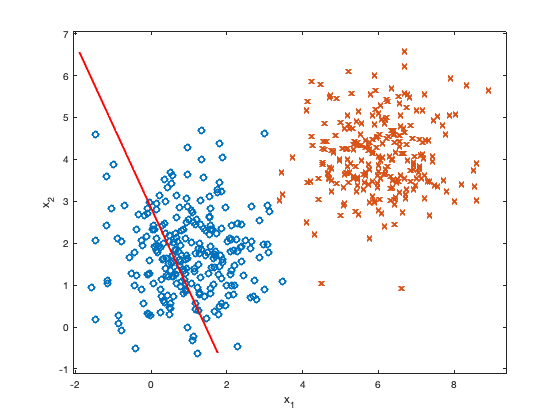
\includegraphics[width=16cm, keepaspectratio]{Initial_Separation_Line_Class}
\end{center}

\begin{center}
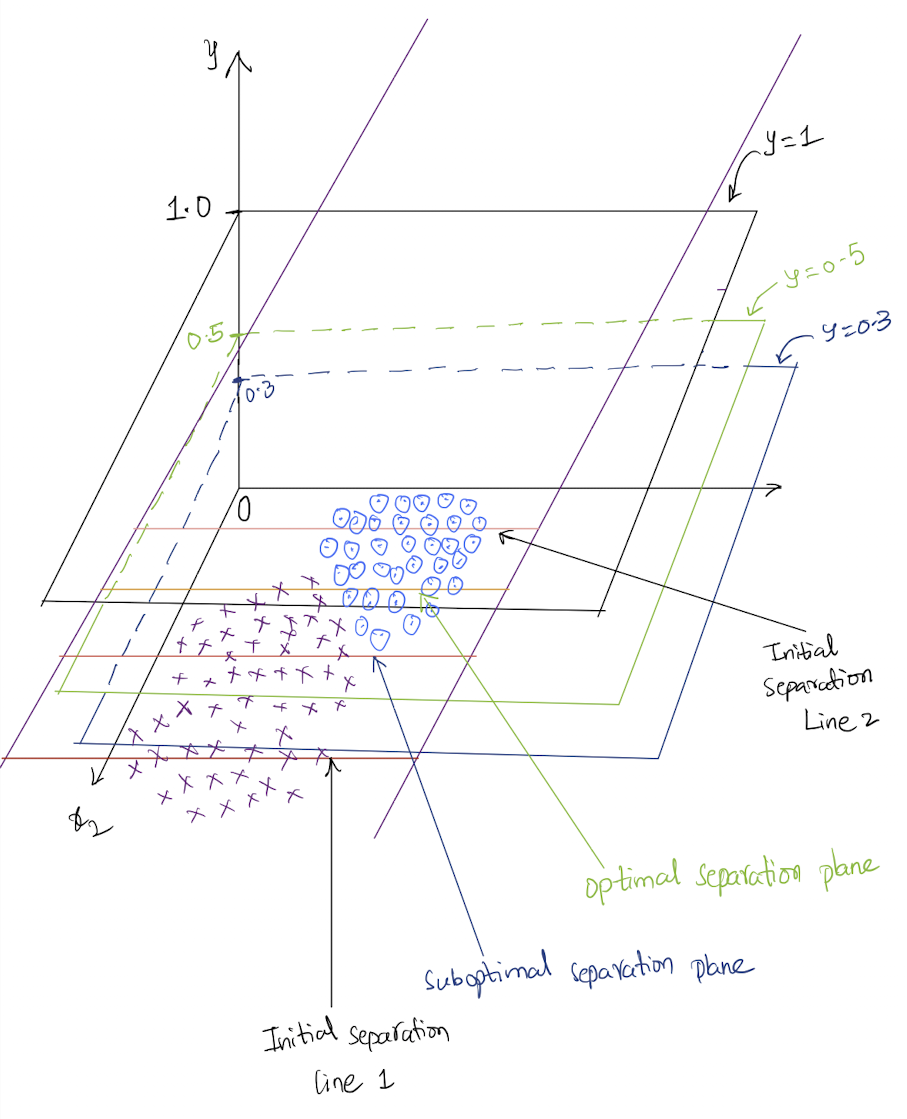
\includegraphics[width=16cm, keepaspectratio]{Problem2}
\end{center}

\subsection*{b)}

However, the above solution can be devised better with a good understanding of the two classes. Instead of taking the separation plane/line as intersection of $\mathbf{w}^{\top} \mathbf{x}=0$ and $y = 0$ (initial separation line 1) or as intersection of $\mathbf{w}^{\top} \mathbf{x}=0$ and $y = 1$ (initial separation line 2), we could take a value that favour both classes equally, i.e., which in this case is intersection of $\mathbf{w}^{\top} \mathbf{x}=0$ and $y = 0.5$ (optimal separation line) as it is in between $y = 0$ and $y = 1$ and more importantly equidistant from the two planes in euclidean space. Intersection with plane such as $y = 0.3$ (suboptimal separation line) would be sub-optimal. This gives a modified initial solution as,

$$
\mathbf{w}^{(0)}=\left(\mathbf{X}^{T} \mathbf{X}\right)^{-1} \mathbf{X}^{T} (\mathbf{y} - 0.5)
$$
where the value $0.5$ above is subtracted from every class label.
\\

The modified line of intersection can be seen as below:

\begin{center}
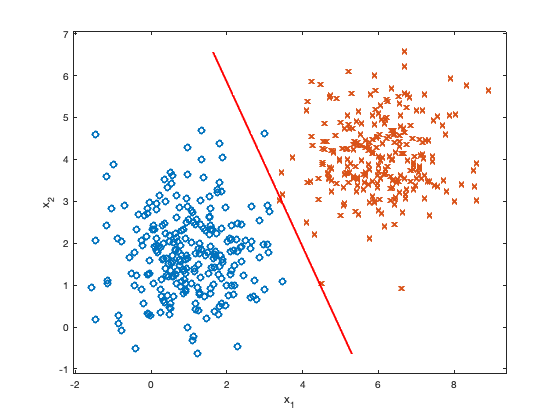
\includegraphics[width=16cm, keepaspectratio]{Final_Separation_Line_Class}
\end{center}

This definitely looks like a better initial solution than the previous one.

c)

In this case, $y \in \{-1, + 1\}$, the mean of the possible class labels is $0$. This means that the solution used in the actual code given on class website should be fine. Hence, we can use,

$$
\mathbf{w}^{(0)}=\left(\mathbf{X}^{T} \mathbf{X}\right)^{-1} \mathbf{X}^{T} \mathbf{y}
$$

\end{solution}


\begin{problem}
Problem 3. (40 points) Consider two classification concepts given in Figure 1 , where $x \in \mathcal{X}=[-6,6] \times$ $[-4,4], y \in \mathcal{Y}=\{-1,+1\}$ and $p(y \mid x) \in\{0,1\}$ is defined in the drawing.

\begin{figure}[H]
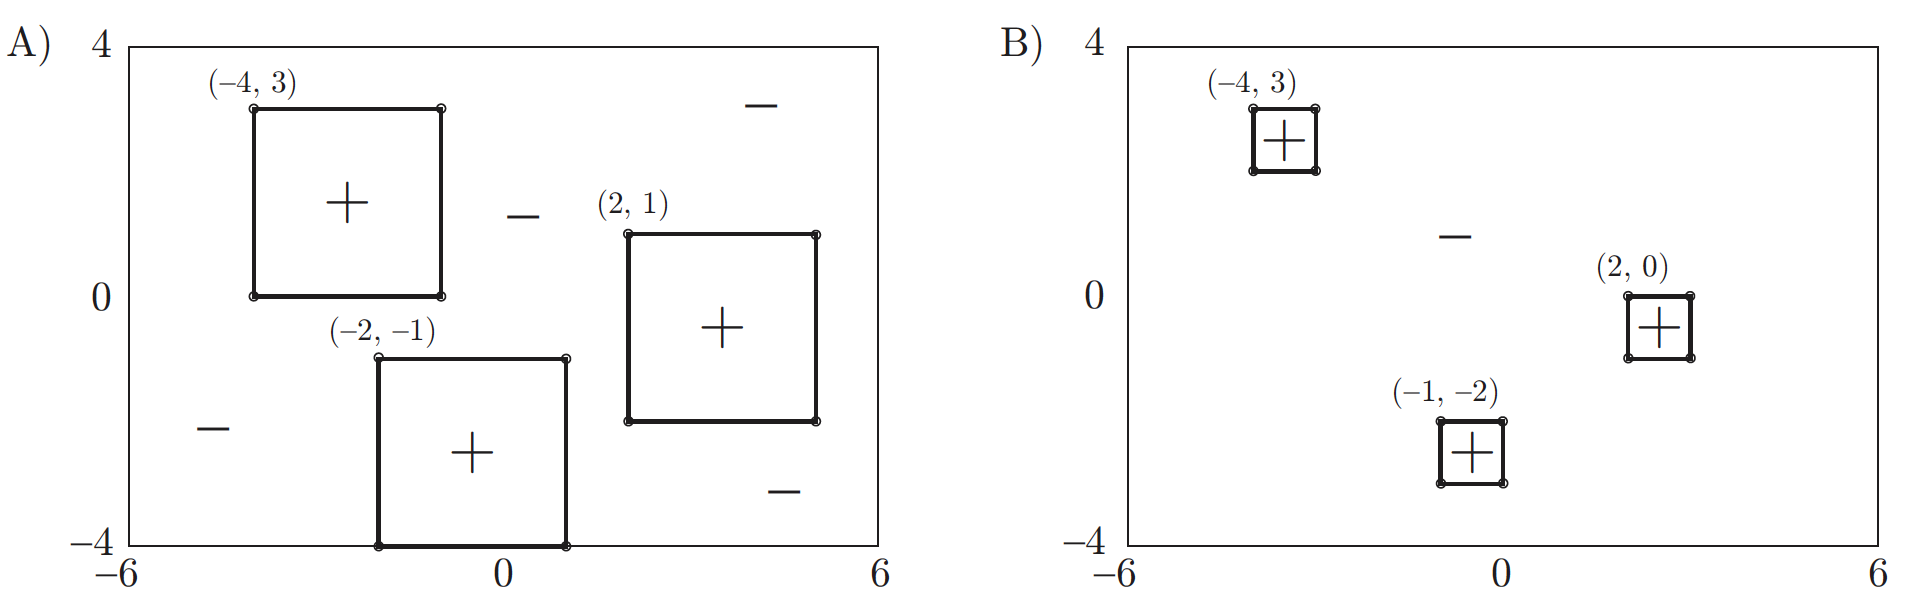
\includegraphics[width=16cm, keepaspectratio]{Problem3}
\caption{Two concepts where examples that fall within any of the three $3 \times 3$ (panel A) or $1 \times 1$ (panel B) squares are labeled positive and the remaining examples (outside each of the squares but within $\mathcal{X}$ ) are labeled negative. The position of the point $x=\left(x_{1}, x_{2}\right)$ in the upper left-hand corner for each square is shown in the picture. Consider horizontal axis to be $x_{1}$ and vertical axis as $x_{2}$.}
\end{figure}


Your experiments in this question will rely on generating a data set of size $n \in\{250,1000,10000\}$ drawn from a uniform distribution in $\mathcal{X}$ and labeled according to the rules from Figure $1 ;$ e.g., $P(Y=1 \mid x)=1$ if $x$ that was randomly drawn is inside any of the three squares in either of the two panels, and $P(Y=1 \mid x)=0$ otherwise. The goal of the following two problems will be to train and evaluate classifiers created from the data generated in this way. You can use any library you want in this assignment and do programming in Python, MATLAB, $R$ or $C / C++$. Your code should be easy to run for each question and sub-question below so that we can replicate your results to the maximum extent possible.

Consider single-output feed-forward neural networks with one or two hidden layers such that the number of hidden neurons in each layer is $h_{1} \in\{1,4,12\}$ and $h_{2} \in\{0,3\},$ respectively, with $h_{2}=0$ meaning that there is no second hidden layer. Consider one of the standard objective functions as your optimization criterion and use early stopping and regularization as needed. Consider a hyperbolic tangent activation function in each neuron and the output but you are free to experiment with others if you'd like to. For each of the architectures, defined by a parameter combination $\left(h_{1}, h_{2}\right),$ evaluate the performance of each model using classification accuracy, balanced accuracy, and area under the ROC curve as your two performance criteria. To evaluate the performance of your models use cross-validation. However, to evaluate the performance of performance evaluation, generate another very large data set on a fine grid in $\mathcal{X} .$ Then use the predictions from your trained model on all these points to determine the "true" performance. You can threshold your predictions in the middle of your prediction range (i.e., at 0.5 if you are predicting between 0 and 1) to determine binary predictions of your models and to then compare those with true class labels you generated on the fine grid.

Provide meaningful comments about all aspects of this exercise (performance results for different network architectures, accuracy of cross-validation, run time, etc.). The comments should not just re-state the results but rather capture trends and give reasoning as to why certain behavior was observed.
\end{problem}

\begin{solution}

For code, please refer to \textbf{NeuralNet.ipynb}.

\subsection*{Results}






\begin{table}[H]
\tiny
\begin{tabular}{|l|l|l|l|l|l|l|l|l|l|l|l|l|l|l|}
\hline
\rowcolor[HTML]{ECF4FF} 
\cellcolor[HTML]{ECF4FF}                        & \cellcolor[HTML]{ECF4FF}                     & \cellcolor[HTML]{ECF4FF}                     & \multicolumn{4}{l|}{\cellcolor[HTML]{ECF4FF}Balanced Accuracy}                                                                    & \multicolumn{4}{l|}{\cellcolor[HTML]{ECF4FF}Classification Accuracy}                                                              & \multicolumn{4}{l|}{\cellcolor[HTML]{ECF4FF}Area Under the ROC Curve}                                                             \\ \cline{4-15} 
\cellcolor[HTML]{ECF4FF}                        & \cellcolor[HTML]{ECF4FF}                     & \cellcolor[HTML]{ECF4FF}                     & \multicolumn{2}{l|}{\cellcolor[HTML]{F8FF00}Uniform}            & \multicolumn{2}{l|}{\cellcolor[HTML]{FFFFC7}Fine}               & \multicolumn{2}{l|}{\cellcolor[HTML]{F8FF00}Uniform}            & \multicolumn{2}{l|}{\cellcolor[HTML]{FFFFC7}Fine}               & \multicolumn{2}{l|}{\cellcolor[HTML]{F8FF00}Uniform}            & \multicolumn{2}{l|}{\cellcolor[HTML]{FFFFC7}Fine}               \\ \cline{4-15} 
\multirow{-3}{*}{\cellcolor[HTML]{ECF4FF}$n$}     & \multirow{-3}{*}{\cellcolor[HTML]{ECF4FF}$h_1$} & \multirow{-3}{*}{\cellcolor[HTML]{ECF4FF}$h_2$} & \cellcolor[HTML]{329A9D}Case A & \cellcolor[HTML]{96FFFB}Case B & \cellcolor[HTML]{329A9D}Case A & \cellcolor[HTML]{96FFFB}Case B & \cellcolor[HTML]{329A9D}Case A & \cellcolor[HTML]{96FFFB}Case B & \cellcolor[HTML]{329A9D}Case A & \cellcolor[HTML]{96FFFB}Case B & \cellcolor[HTML]{329A9D}Case A & \cellcolor[HTML]{96FFFB}Case B & \cellcolor[HTML]{329A9D}Case A & \cellcolor[HTML]{96FFFB}Case B \\ \hline
\rowcolor[HTML]{C0C0C0} 
\cellcolor[HTML]{9AFF99}                        & \cellcolor[HTML]{FE0000}                     & \cellcolor[HTML]{FFCE93}0                    & 0.5                            & 0.5                            & 0.5                            & 0.5                            & \cellcolor[HTML]{EFEFEF}0.72   & \cellcolor[HTML]{EFEFEF}0.964  & \cellcolor[HTML]{EFEFEF}0.7188 & \cellcolor[HTML]{EFEFEF}0.9688 & 0.5645                         & 0.4226                         & 0.5992                         & 0.5025                         \\ \cline{3-15} 
\rowcolor[HTML]{EFEFEF} 
\cellcolor[HTML]{9AFF99}                        & \multirow{-2}{*}{\cellcolor[HTML]{FE0000}1}  & \cellcolor[HTML]{F8A102}3                    & 0.5                            & 0.5                            & 0.5468                         & 0.5                            & \cellcolor[HTML]{C0C0C0}0.72   & \cellcolor[HTML]{C0C0C0}0.964  & \cellcolor[HTML]{C0C0C0}0.7164 & \cellcolor[HTML]{C0C0C0}0.9688 & 0.4991                         & 0.4676                         & 0.688                          & 0.5117                         \\ \cline{2-15} 
\rowcolor[HTML]{C0C0C0} 
\cellcolor[HTML]{9AFF99}                        & \cellcolor[HTML]{FD6864}                     & \cellcolor[HTML]{FFCE93}0                    & 0.5714                         & 0.5                            & 0.5891                         & 0.5                            & \cellcolor[HTML]{EFEFEF}0.716  & \cellcolor[HTML]{EFEFEF}0.964  & \cellcolor[HTML]{EFEFEF}0.7516 & \cellcolor[HTML]{EFEFEF}0.9688 & 0.7624                         & 0.447                          & 0.7611                         & 0.6907                         \\ \cline{3-15} 
\rowcolor[HTML]{EFEFEF} 
\cellcolor[HTML]{9AFF99}                        & \multirow{-2}{*}{\cellcolor[HTML]{FD6864}4}  & \cellcolor[HTML]{F8A102}3                    & 0.7403                         & 0.5                            & 0.7262                         & 0.517                          & \cellcolor[HTML]{C0C0C0}0.84   & \cellcolor[HTML]{C0C0C0}0.964  & \cellcolor[HTML]{C0C0C0}0.8296 & \cellcolor[HTML]{C0C0C0}0.9679 & 0.876                          & 0.5582                         & 0.8869                         & 0.7826                         \\ \cline{2-15} 
\rowcolor[HTML]{C0C0C0} 
\cellcolor[HTML]{9AFF99}                        & \cellcolor[HTML]{FFCCC9}                     & \cellcolor[HTML]{FFCE93}0                    & 0.8258                         & 0.598                          & 0.8421                         & 0.4994                         & \cellcolor[HTML]{EFEFEF}0.888  & \cellcolor[HTML]{EFEFEF}0.964  & \cellcolor[HTML]{EFEFEF}0.8868 & \cellcolor[HTML]{EFEFEF}0.9676 & 0.9592                         & 0.8097                         & 0.9498                         & 0.7132                         \\ \cline{3-15} 
\rowcolor[HTML]{EFEFEF} 
\multirow{-6}{*}{\cellcolor[HTML]{9AFF99}250}   & \multirow{-2}{*}{\cellcolor[HTML]{FFCCC9}12} & \cellcolor[HTML]{F8A102}3                    & 0.925                          & 0.5939                         & 0.8756                         & 0.5378                         & \cellcolor[HTML]{C0C0C0}0.936  & \cellcolor[HTML]{C0C0C0}0.956  & \cellcolor[HTML]{C0C0C0}0.9047 & \cellcolor[HTML]{C0C0C0}0.9651 & 0.9806                         & 0.6856                         & 0.9465                         & 0.7522                         \\ \hline
\rowcolor[HTML]{C0C0C0} 
\cellcolor[HTML]{32CB00}                        & \cellcolor[HTML]{FE0000}                     & \cellcolor[HTML]{FFCE93}0                    & 0.5                            & 0.5                            & 0.5                            & 0.5                            & \cellcolor[HTML]{EFEFEF}0.73   & \cellcolor[HTML]{EFEFEF}0.973  & \cellcolor[HTML]{EFEFEF}0.7188 & \cellcolor[HTML]{EFEFEF}0.9688 & 0.5784                         & 0.3753                         & 0.4915                         & 0.4966                         \\ \cline{3-15} 
\rowcolor[HTML]{EFEFEF} 
\cellcolor[HTML]{32CB00}                        & \multirow{-2}{*}{\cellcolor[HTML]{FE0000}1}  & \cellcolor[HTML]{F8A102}3                    & 0.5                            & 0.5                            & 0.597                          & 0.5                            & \cellcolor[HTML]{C0C0C0}0.73   & \cellcolor[HTML]{C0C0C0}0.973  & \cellcolor[HTML]{C0C0C0}0.7539 & \cellcolor[HTML]{C0C0C0}0.9688 & 0.6095                         & 0.563                          & 0.7428                         & 0.5052                         \\ \cline{2-15} 
\rowcolor[HTML]{C0C0C0} 
\cellcolor[HTML]{32CB00}                        & \cellcolor[HTML]{FD6864}                     & \cellcolor[HTML]{FFCE93}0                    & 0.633                          & 0.5                            & 0.6404                         & 0.5                            & \cellcolor[HTML]{EFEFEF}0.779  & \cellcolor[HTML]{EFEFEF}0.973  & \cellcolor[HTML]{EFEFEF}0.7832 & \cellcolor[HTML]{EFEFEF}0.9688 & 0.78                           & 0.4325                         & 0.8282                         & 0.6443                         \\ \cline{3-15} 
\rowcolor[HTML]{EFEFEF} 
\cellcolor[HTML]{32CB00}                        & \multirow{-2}{*}{\cellcolor[HTML]{FD6864}4}  & \cellcolor[HTML]{F8A102}3                    & 0.7083                         & 0.5                            & 0.7846                         & 0.5                            & \cellcolor[HTML]{C0C0C0}0.813  & \cellcolor[HTML]{C0C0C0}0.973  & \cellcolor[HTML]{C0C0C0}0.8505 & \cellcolor[HTML]{C0C0C0}0.9688 & 0.8764                         & 0.4511                         & 0.9223                         & 0.4485                         \\ \cline{2-15} 
\rowcolor[HTML]{C0C0C0} 
\cellcolor[HTML]{32CB00}                        & \cellcolor[HTML]{FFCCC9}                     & \cellcolor[HTML]{FFCE93}0                    & 0.7919                         & 0.5                            & 0.8056                         & 0.5                            & \cellcolor[HTML]{EFEFEF}0.859  & \cellcolor[HTML]{EFEFEF}0.973  & \cellcolor[HTML]{EFEFEF}0.8734 & \cellcolor[HTML]{EFEFEF}0.9688 & 0.9246                         & 0.8589                         & 0.9528                         & 0.8417                         \\ \cline{3-15} 
\rowcolor[HTML]{EFEFEF} 
\multirow{-6}{*}{\cellcolor[HTML]{32CB00}1000}  & \multirow{-2}{*}{\cellcolor[HTML]{FFCCC9}12} & \cellcolor[HTML]{F8A102}3                    & 0.9233                         & 0.5662                         & 0.8846                         & 0.5                            & \cellcolor[HTML]{C0C0C0}0.948  & \cellcolor[HTML]{C0C0C0}0.974  & \cellcolor[HTML]{C0C0C0}0.9206 & \cellcolor[HTML]{C0C0C0}0.9688 & 0.9857                         & 0.5164                         & 0.9708                         & 0.504                          \\ \hline
\rowcolor[HTML]{C0C0C0} 
\cellcolor[HTML]{009901}                        & \cellcolor[HTML]{FE0000}                     & \cellcolor[HTML]{FFCE93}0                    & 0.5                            & 0.5                            & 0.5                            & 0.5                            & \cellcolor[HTML]{EFEFEF}0.7184 & \cellcolor[HTML]{EFEFEF}0.9699 & \cellcolor[HTML]{EFEFEF}0.7188 & \cellcolor[HTML]{EFEFEF}0.9688 & 0.5895                         & 0.4685                         & 0.4982                         & 0.5156                         \\ \cline{3-15} 
\rowcolor[HTML]{EFEFEF} 
\cellcolor[HTML]{009901}                        & \multirow{-2}{*}{\cellcolor[HTML]{FE0000}1}  & \cellcolor[HTML]{F8A102}3                    & 0.5                            & 0.5                            & 0.5                            & 0.5                            & \cellcolor[HTML]{C0C0C0}0.7184 & \cellcolor[HTML]{C0C0C0}0.9699 & \cellcolor[HTML]{C0C0C0}0.7188 & \cellcolor[HTML]{C0C0C0}0.9688 & 0.6229                         & 0.5404                         & 0.6598                         & 0.5215                         \\ \cline{2-15} 
\rowcolor[HTML]{C0C0C0} 
\cellcolor[HTML]{009901}                        & \cellcolor[HTML]{FD6864}                     & \cellcolor[HTML]{FFCE93}0                    & 0.6286                         & 0.5                            & 0.6506                         & 0.5                            & \cellcolor[HTML]{EFEFEF}0.7853 & \cellcolor[HTML]{EFEFEF}0.9699 & \cellcolor[HTML]{EFEFEF}0.7771 & \cellcolor[HTML]{EFEFEF}0.9688 & 0.6932                         & 0.5407                         & 0.8395                         & 0.613                          \\ \cline{3-15} 
\rowcolor[HTML]{EFEFEF} 
\cellcolor[HTML]{009901}                        & \multirow{-2}{*}{\cellcolor[HTML]{FD6864}4}  & \cellcolor[HTML]{F8A102}3                    & 0.755                          & 0.5                            & 0.8019                         & 0.5                            & \cellcolor[HTML]{C0C0C0}0.8325 & \cellcolor[HTML]{C0C0C0}0.9699 & \cellcolor[HTML]{C0C0C0}0.8523 & \cellcolor[HTML]{C0C0C0}0.9688 & 0.8894                         & 0.5129                         & 0.9048                         & 0.7529                         \\ \cline{2-15} 
\rowcolor[HTML]{C0C0C0} 
\cellcolor[HTML]{009901}                        & \cellcolor[HTML]{FFCCC9}                     & \cellcolor[HTML]{FFCE93}0                    & 0.8703                         & 0.5085                         & 0.8175                         & 0.5                            & \cellcolor[HTML]{EFEFEF}0.9031 & \cellcolor[HTML]{EFEFEF}0.9704 & \cellcolor[HTML]{EFEFEF}0.8709 & \cellcolor[HTML]{EFEFEF}0.9688 & 0.9601                         & 0.8795                         & 0.9412                         & 0.7865                         \\ \cline{3-15} 
\rowcolor[HTML]{EFEFEF} 
\multirow{-6}{*}{\cellcolor[HTML]{009901}10000} & \multirow{-2}{*}{\cellcolor[HTML]{FFCCC9}12} & \cellcolor[HTML]{F8A102}3                    & 0.9354                         & 0.5                            & 0.9271                         & 0.6089                         & \cellcolor[HTML]{C0C0C0}0.9514 & \cellcolor[HTML]{C0C0C0}0.9699 & \cellcolor[HTML]{C0C0C0}0.9455 & \cellcolor[HTML]{C0C0C0}0.9741 & 0.9879                         & 0.5582                         & 0.9857                         & 0.8204                         \\ \hline
\end{tabular}
\end{table}





\subsection*{Setup}

A single-output feed-forward neural network with one/two hidden layers is modelled such that the number of hidden neurons in each hidden layer is $h_1 \in \{1, 4, 12\}$ and $h_2 \in \{0, 3\}$, respectively, with $h_2 = 0$ meaning that there is no second hidden layer. I used binary cross-entropy standard objective function as my optimization criterion. I ran the model for 1000 epochs (configurable hyperparameter). I used Adam optimizer in order to converge to a local optimum. There is no other early stopping criterion in my training. I prefer to use regularization only for $y$. I map $y = -1 \text{ to } y = 0$ and $y = 1 \text{ to } y = 1$. There is no regularization for $X$ as the data set values are mostly comparable and picked from a uniform distribution from $[-6, 6] \text{ and } [-4, 4]$ respectively. The expected mean is any way zero and the variance is low. I also don't see any threat of outliers. I didn't use any special initialization for weights. I went with default initialization provided by PyTorch which is choosing weights from \textbf{Uniform Distribution} from $\left(-\frac{1}{\sqrt{d}}, \frac{1}{\sqrt{d}}\right)$, where $d$ is the number of features. I used a hyperbolic tangent ($tanh$) activation function in each activation. The output layer is estimated using sigmoid function and the threshold I used to classify negatives and positives is 0.5. For each of the architectures, defined by a parameter combination $(h_1, h_2)$, I evaluated the performance of each model using balanced accuracy, classification accuracy, and area under the ROC curve. These are the outputs of my function $get\_metrics$. To evaluate the performance of my model, I used $k$-fold stratified cross-validation (with $k = 5$) by splitting the sample into $80-20$ ($80$ for training and $20$ for testing). To evaluate the performance of performance evaluation, I generated another very large dataset on a fine grid in X. The points in this grid are spaced at intervals of $0.1$ both horizontally and vertically. I calculated the predictions from my trained model on all these points to determine the true performance. In order to calculate the classification accuracy and balanced accuracy, I used the thresholded predictions and to calculate the area under the curve I used soft predictions.

In the above table, the columns are appropriately named. 'Uniform' refers to values obtained from uniform distribution and 'Fine' refers to data from fine grid (spaced at $0.1$). 'Case A' refers to relatively balanced case and 'Case B' refers to highly imbalanced case. The coloring of columns $n$, $h_1$, and $h_2$ are mapped as per the expected performance of the model.


\subsection*{Plots}

\begin{figure}[H]
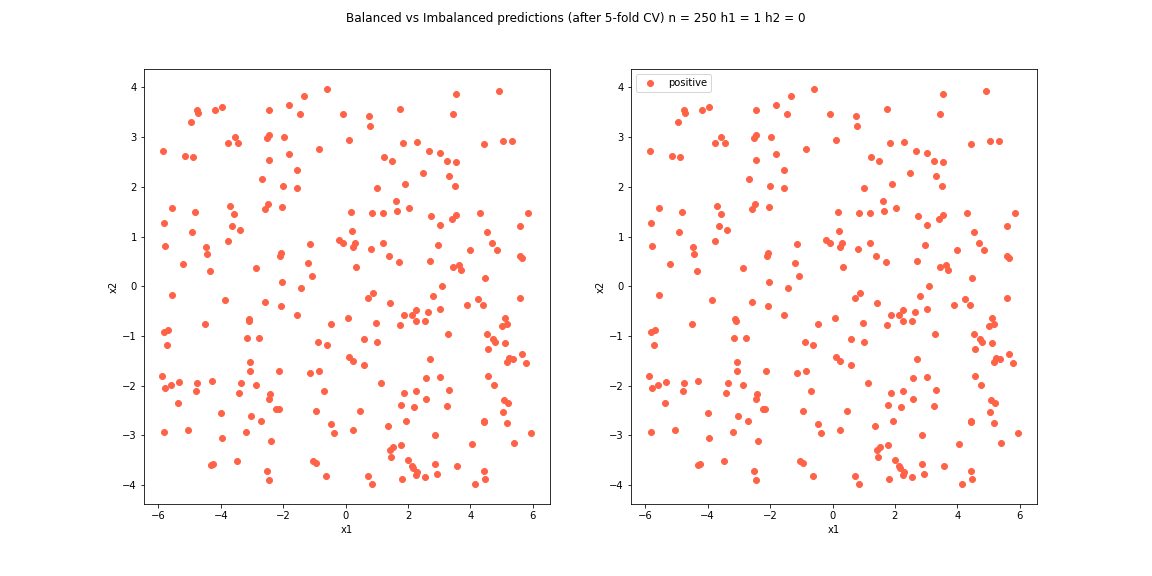
\includegraphics[width=16cm, keepaspectratio]{./3/1}
\end{figure}
\begin{figure}[H]
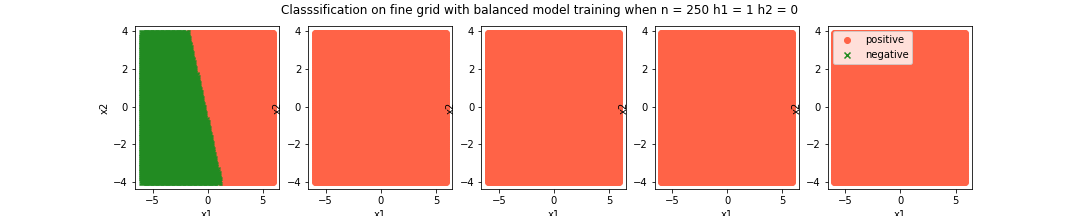
\includegraphics[width=16cm, keepaspectratio]{./3/2}
\end{figure}
\begin{figure}[H]
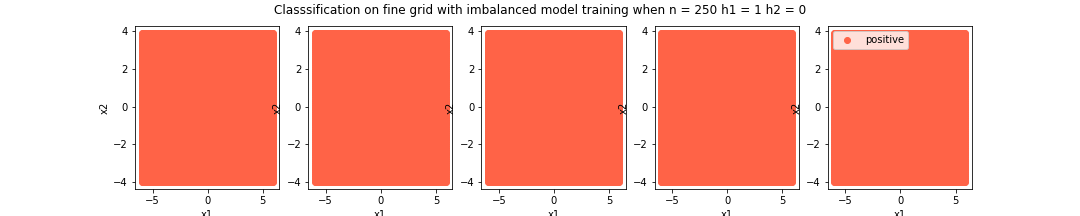
\includegraphics[width=16cm, keepaspectratio]{./3/3}
\end{figure}
\begin{figure}[H]
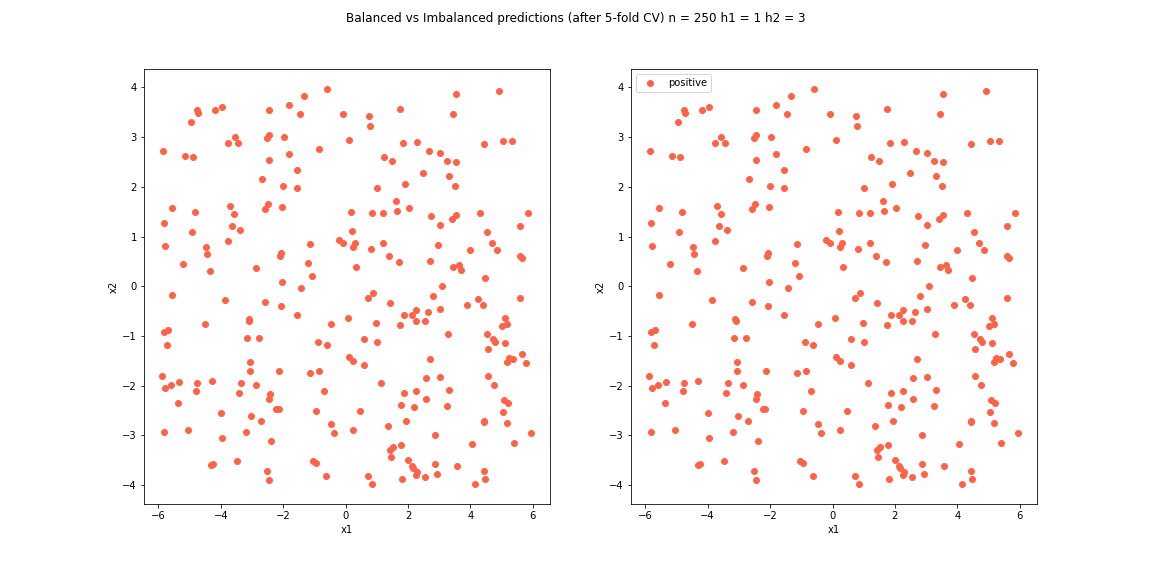
\includegraphics[width=16cm, keepaspectratio]{./3/4}
\end{figure}
\begin{figure}[H]
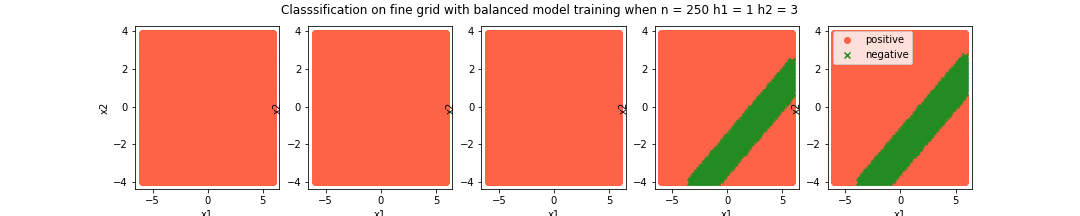
\includegraphics[width=16cm, keepaspectratio]{./3/5}
\end{figure}
\begin{figure}[H]
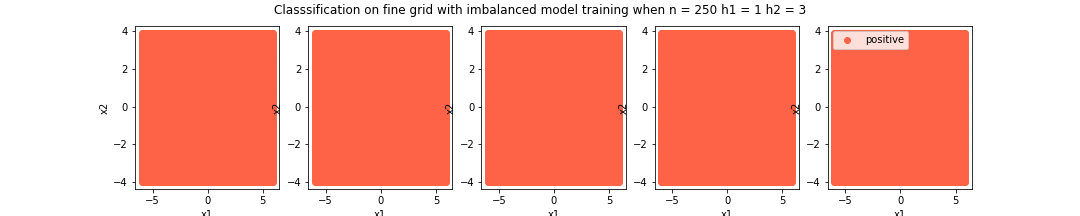
\includegraphics[width=16cm, keepaspectratio]{./3/6}
\end{figure}
\begin{figure}[H]
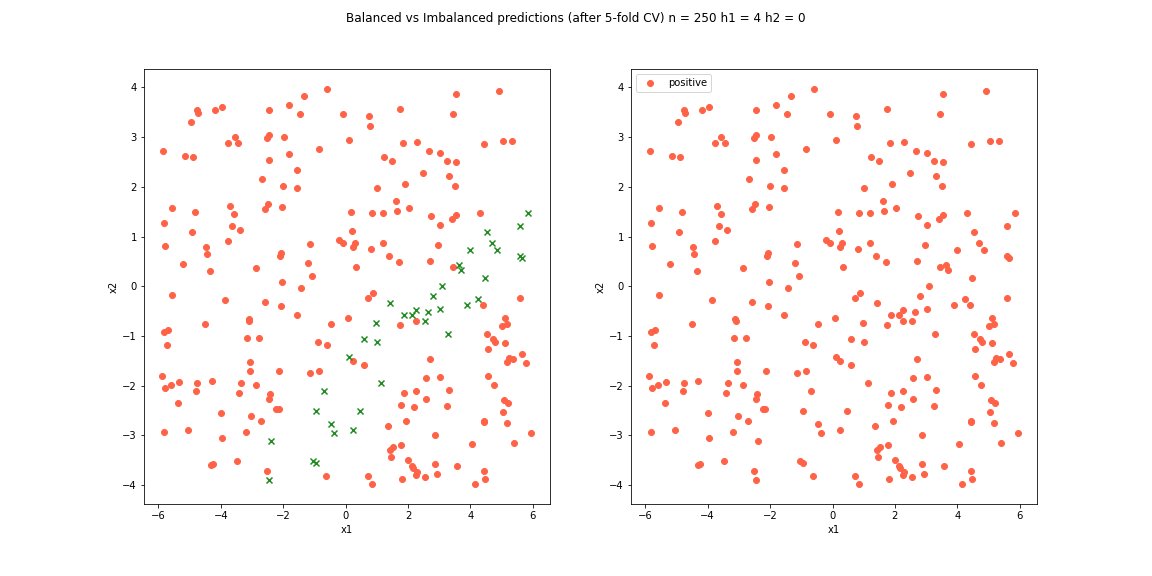
\includegraphics[width=16cm, keepaspectratio]{./3/7}
\end{figure}
\begin{figure}[H]
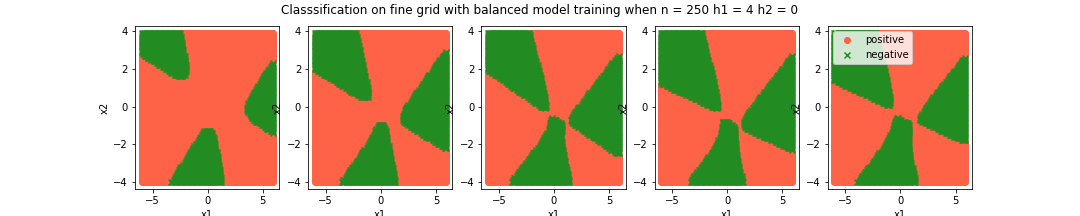
\includegraphics[width=16cm, keepaspectratio]{./3/8}
\end{figure}
\begin{figure}[H]
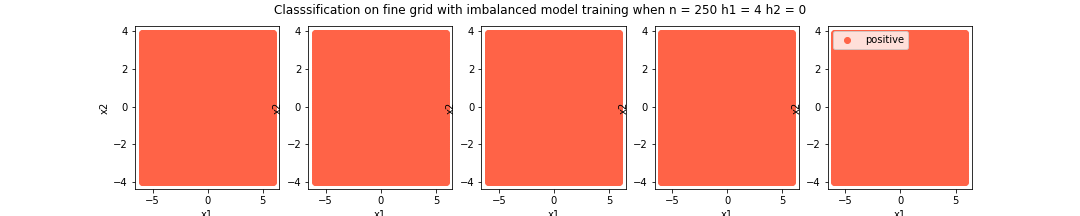
\includegraphics[width=16cm, keepaspectratio]{./3/9}
\end{figure}
\begin{figure}[H]
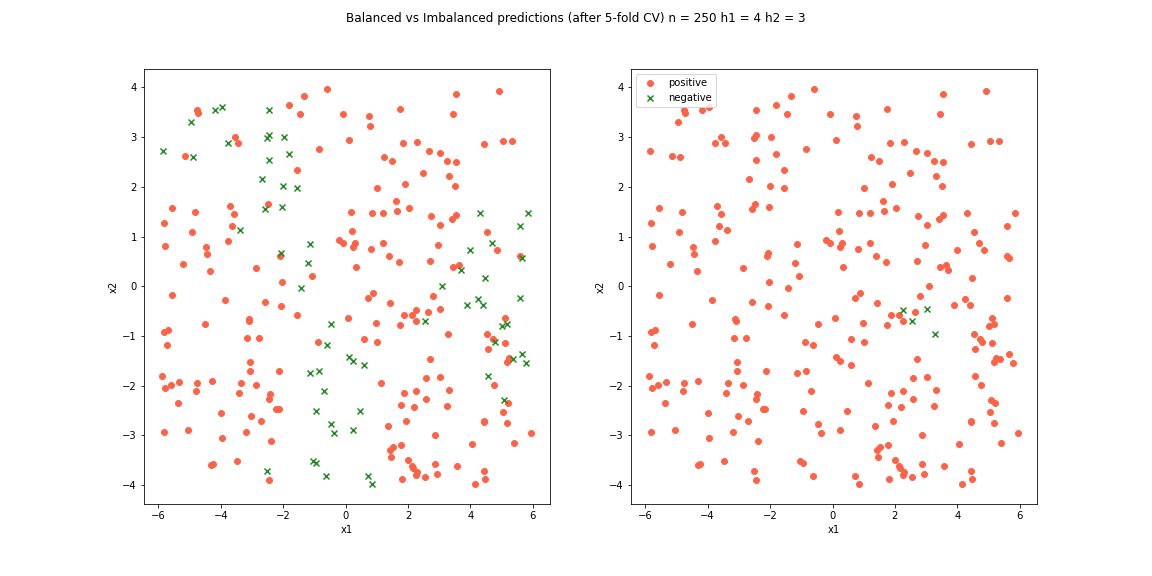
\includegraphics[width=16cm, keepaspectratio]{./3/10}
\end{figure}
\begin{figure}[H]
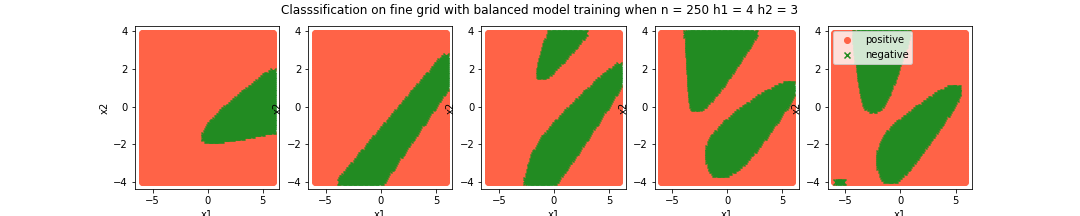
\includegraphics[width=16cm, keepaspectratio]{./3/11}
\end{figure}
\begin{figure}[H]
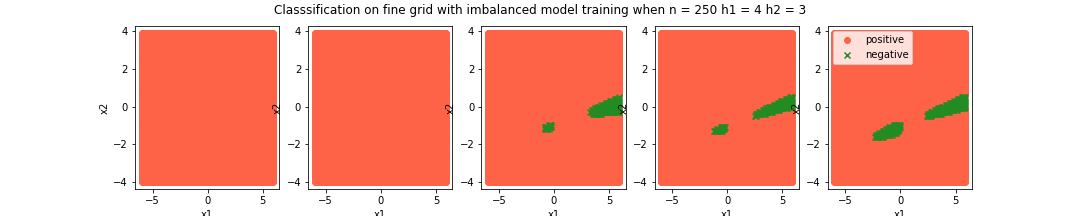
\includegraphics[width=16cm, keepaspectratio]{./3/12}
\end{figure}
\begin{figure}[H]
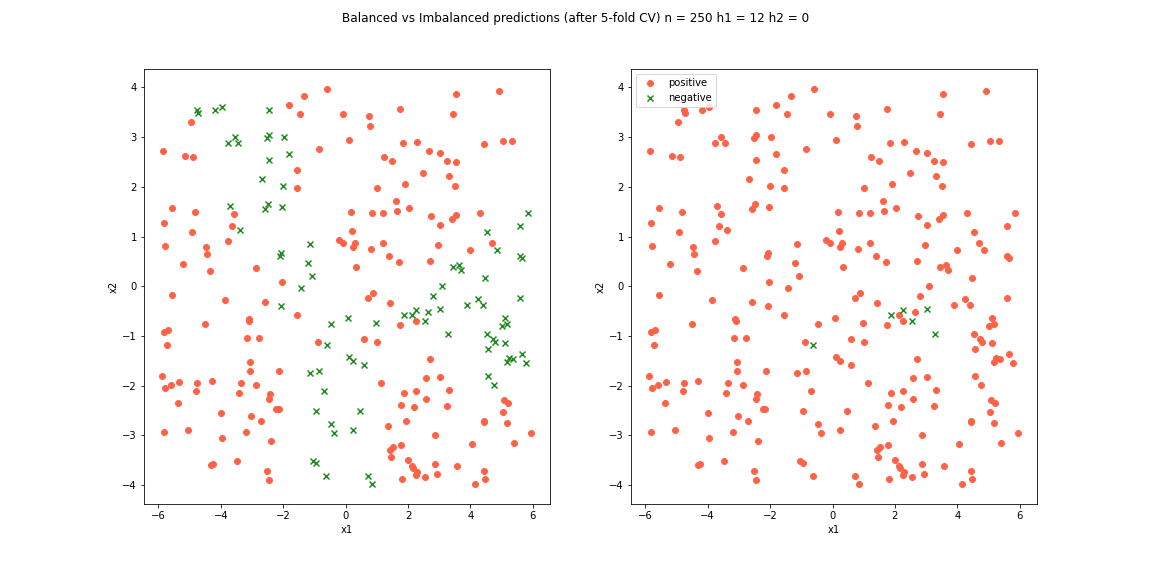
\includegraphics[width=16cm, keepaspectratio]{./3/13}
\end{figure}
\begin{figure}[H]
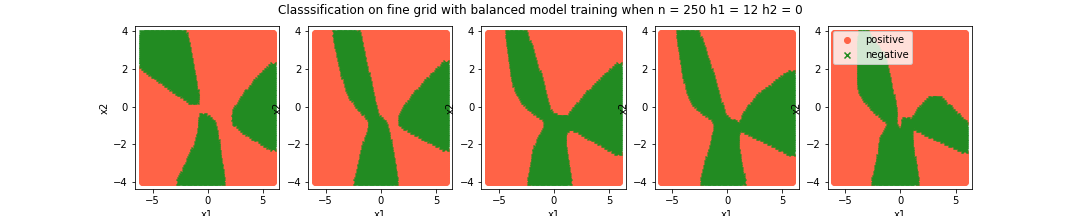
\includegraphics[width=16cm, keepaspectratio]{./3/14}
\end{figure}
\begin{figure}[H]
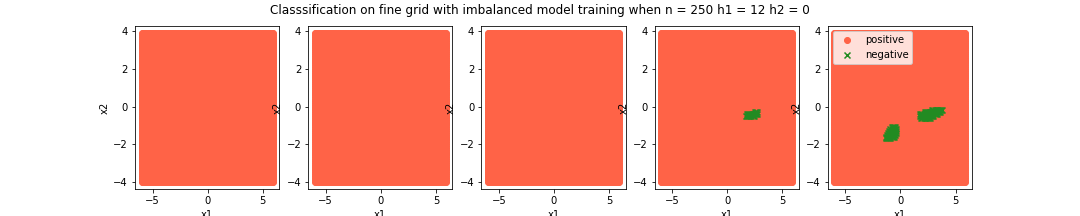
\includegraphics[width=16cm, keepaspectratio]{./3/15}
\end{figure}
\begin{figure}[H]
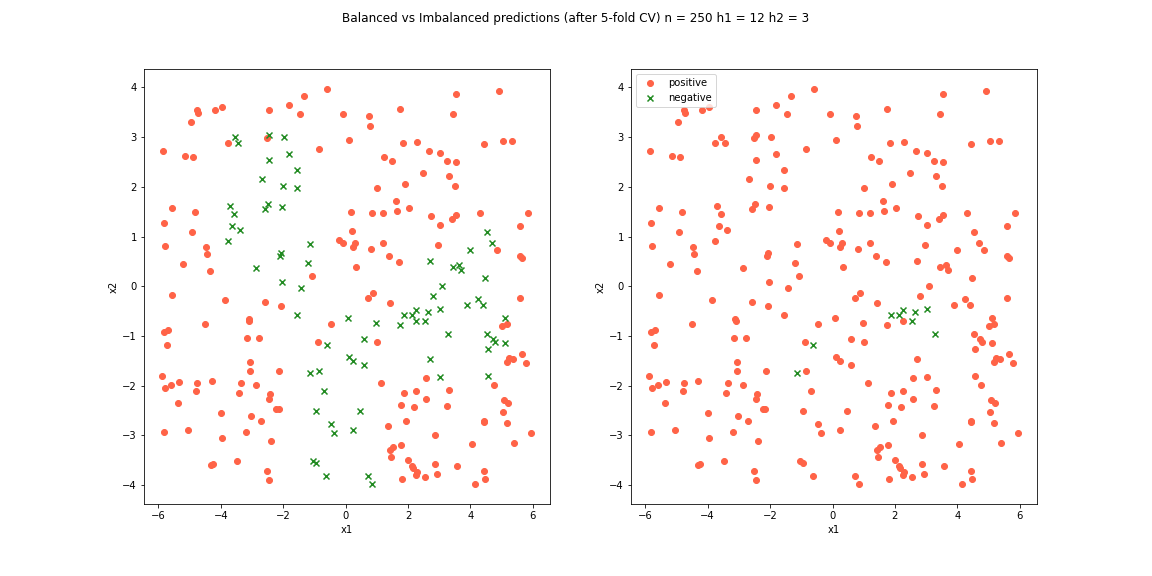
\includegraphics[width=16cm, keepaspectratio]{./3/16}
\end{figure}
\begin{figure}[H]
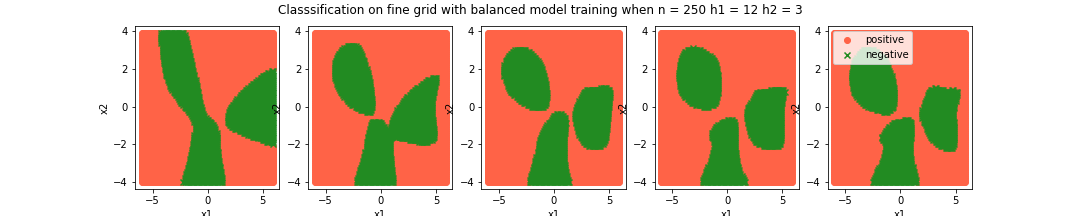
\includegraphics[width=16cm, keepaspectratio]{./3/17}
\end{figure}
\begin{figure}[H]
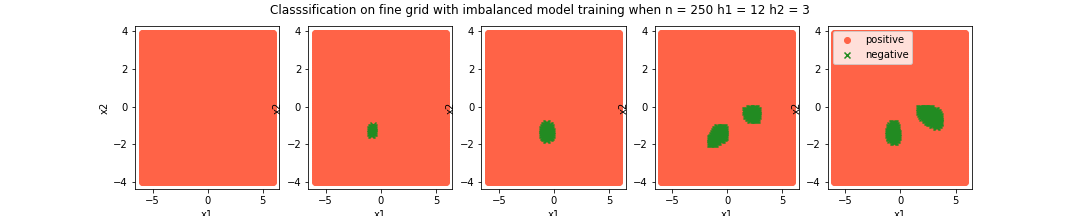
\includegraphics[width=16cm, keepaspectratio]{./3/18}
\end{figure}
\begin{figure}[H]
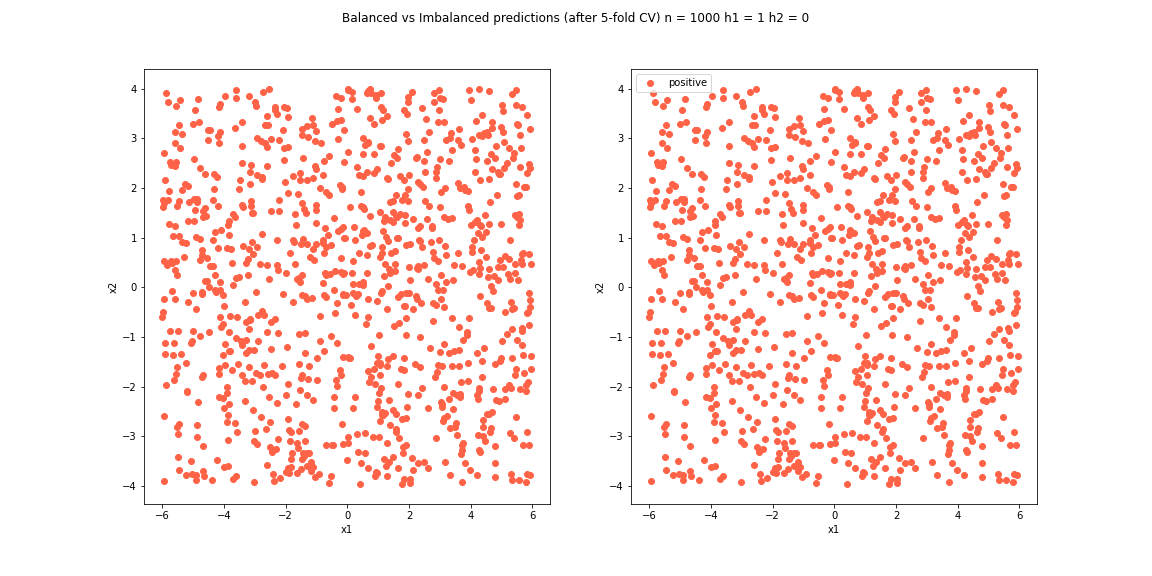
\includegraphics[width=16cm, keepaspectratio]{./3/19}
\end{figure}
\begin{figure}[H]
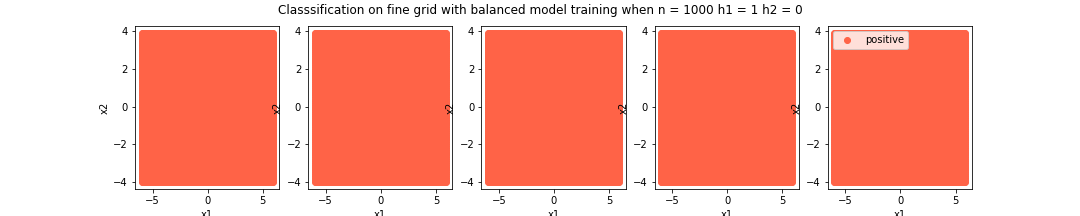
\includegraphics[width=16cm, keepaspectratio]{./3/20}
\end{figure}
\begin{figure}[H]
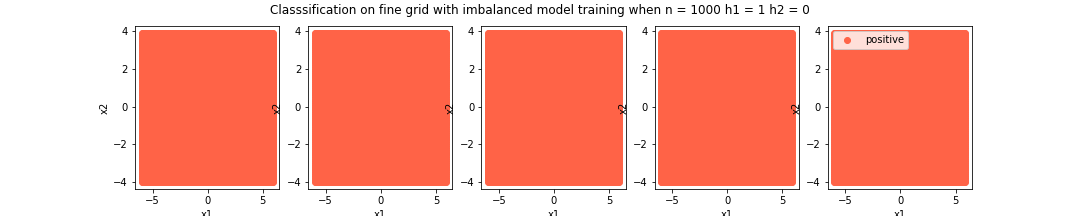
\includegraphics[width=16cm, keepaspectratio]{./3/21}
\end{figure}
\begin{figure}[H]
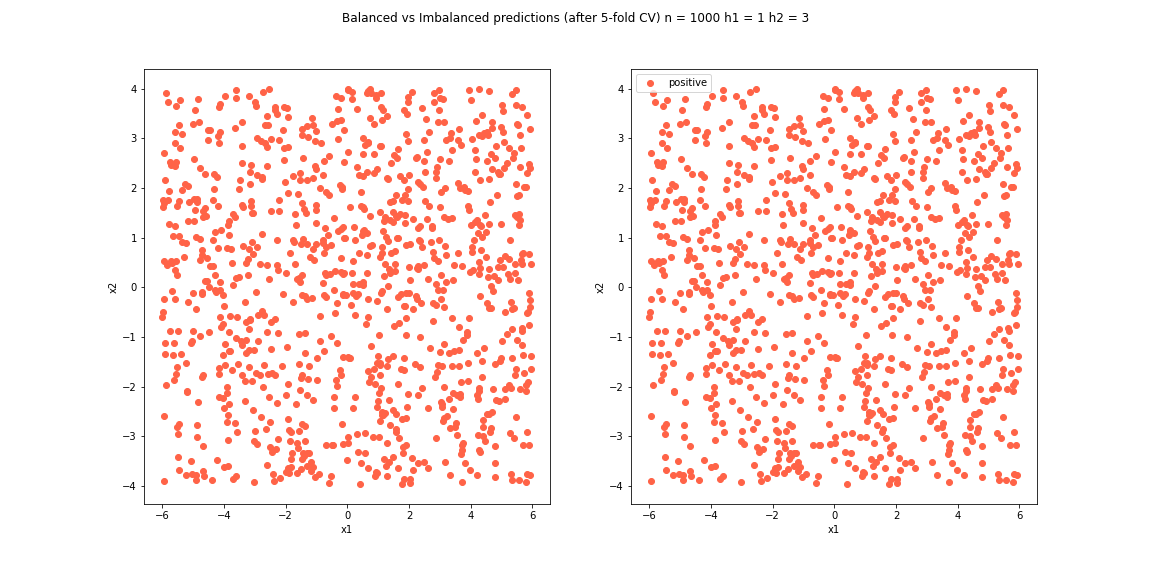
\includegraphics[width=16cm, keepaspectratio]{./3/22}
\end{figure}
\begin{figure}[H]
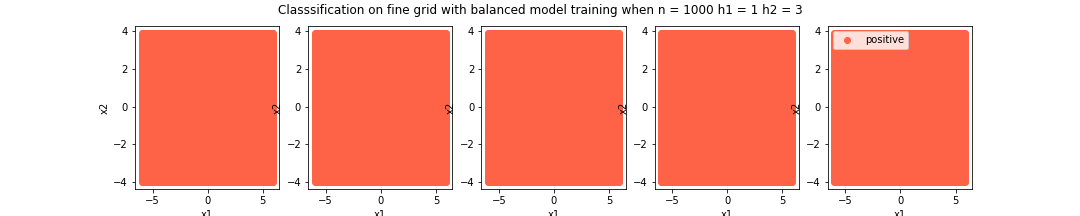
\includegraphics[width=16cm, keepaspectratio]{./3/23}
\end{figure}
\begin{figure}[H]
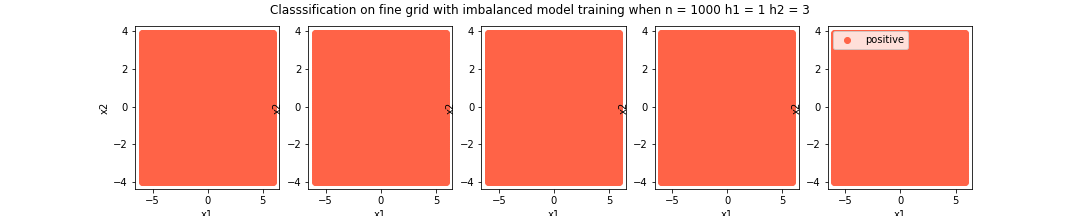
\includegraphics[width=16cm, keepaspectratio]{./3/24}
\end{figure}
\begin{figure}[H]
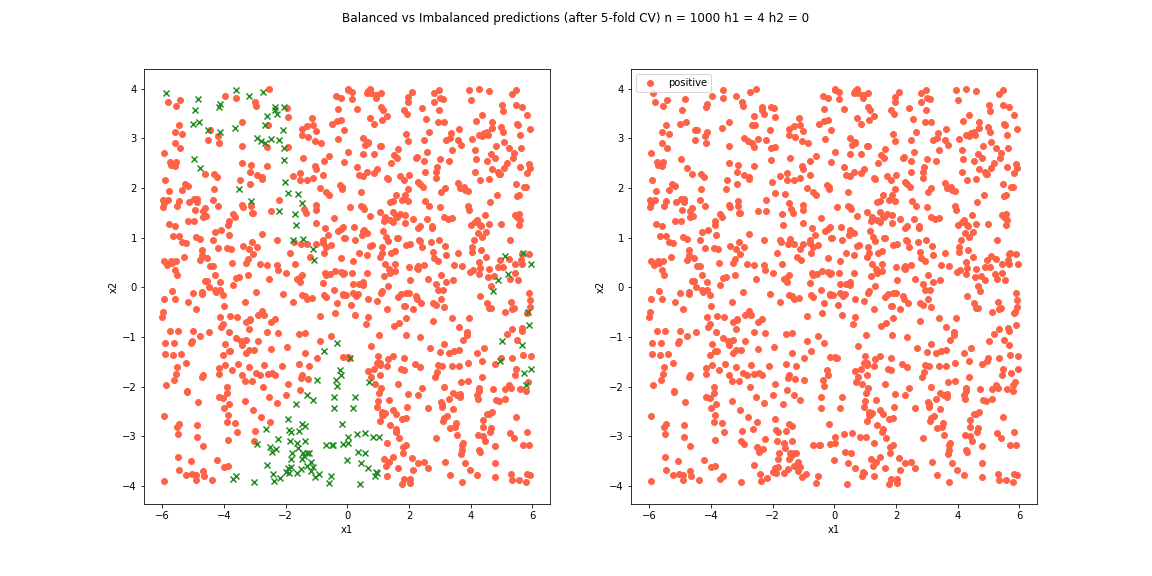
\includegraphics[width=16cm, keepaspectratio]{./3/25}
\end{figure}
\begin{figure}[H]
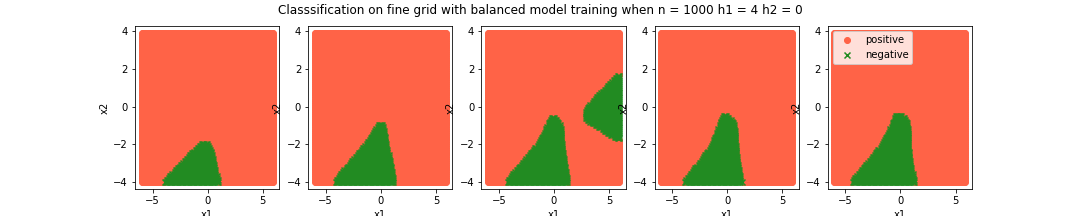
\includegraphics[width=16cm, keepaspectratio]{./3/26}
\end{figure}
\begin{figure}[H]
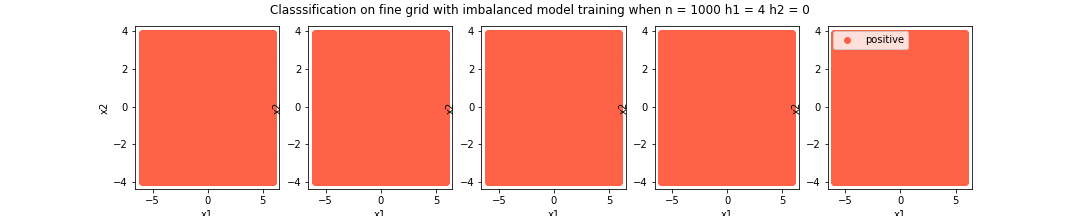
\includegraphics[width=16cm, keepaspectratio]{./3/27}
\end{figure}
\begin{figure}[H]
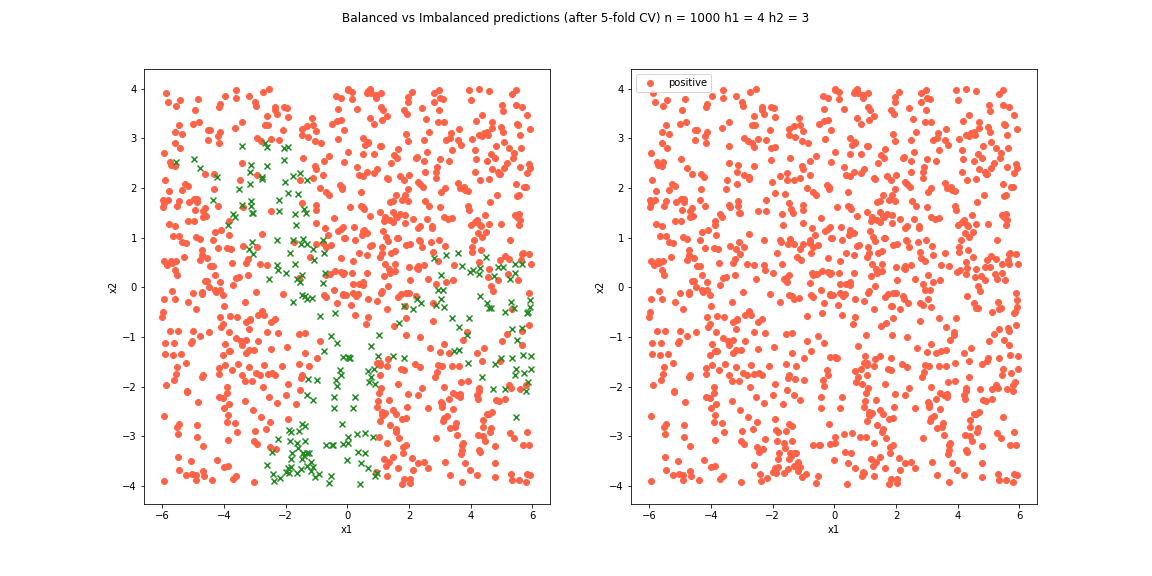
\includegraphics[width=16cm, keepaspectratio]{./3/28}
\end{figure}
\begin{figure}[H]
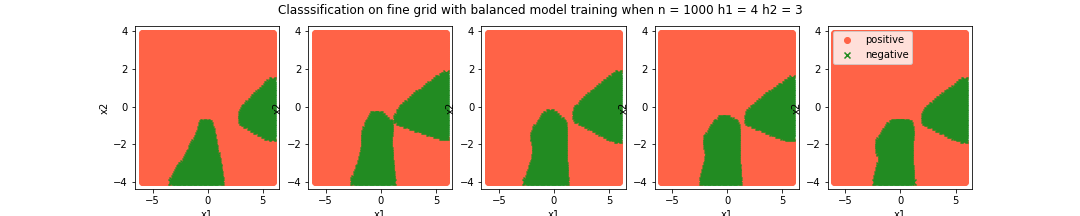
\includegraphics[width=16cm, keepaspectratio]{./3/29}
\end{figure}
\begin{figure}[H]
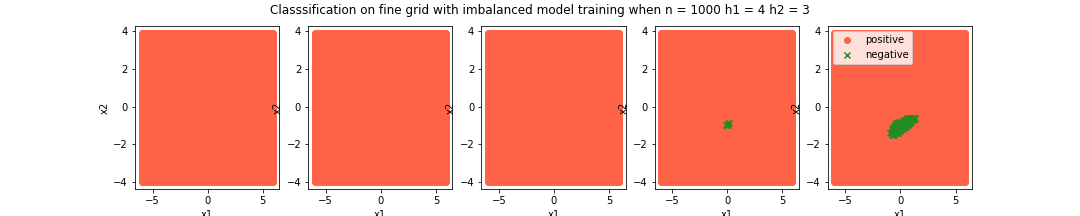
\includegraphics[width=16cm, keepaspectratio]{./3/30}
\end{figure}
\begin{figure}[H]
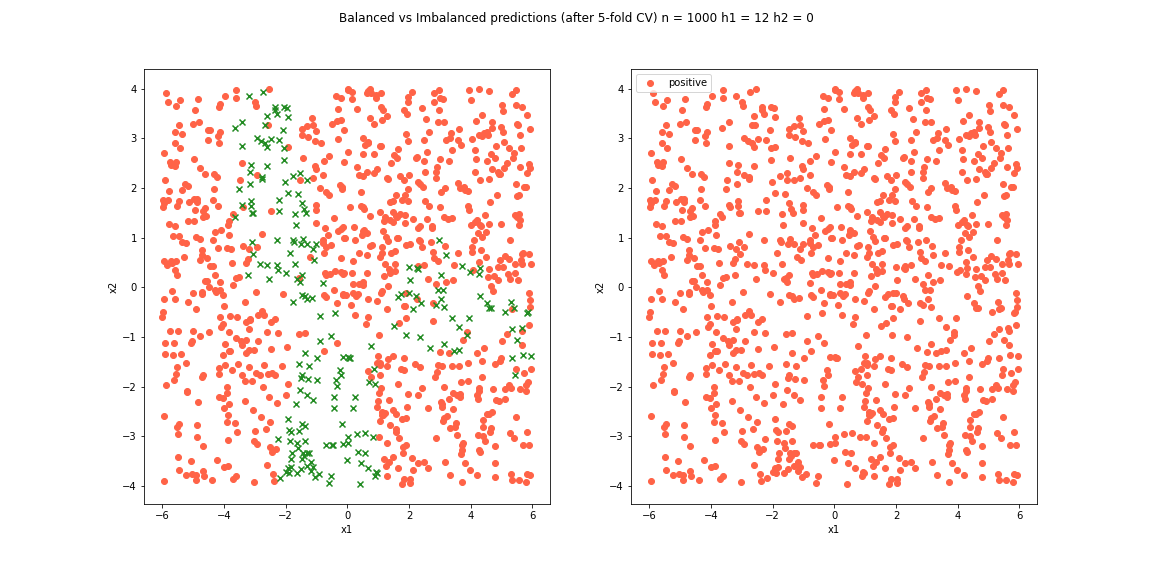
\includegraphics[width=16cm, keepaspectratio]{./3/31}
\end{figure}
\begin{figure}[H]
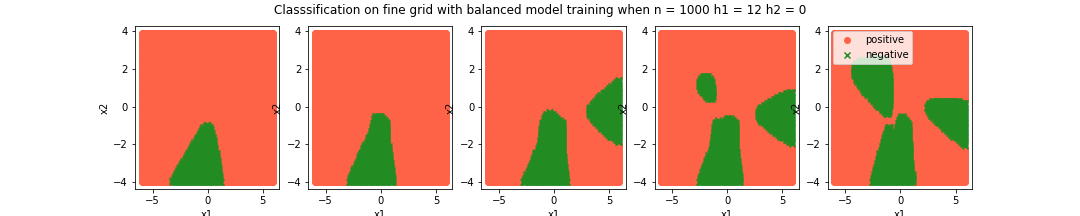
\includegraphics[width=16cm, keepaspectratio]{./3/32}
\end{figure}
\begin{figure}[H]
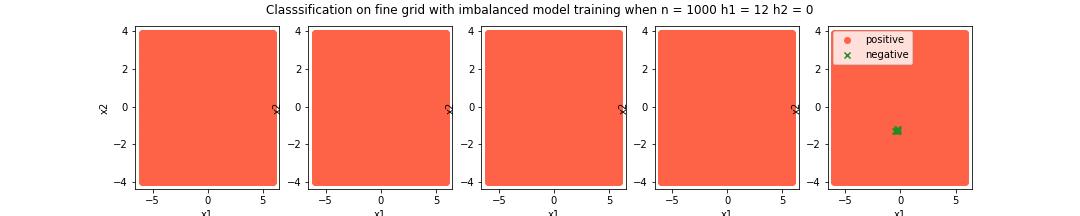
\includegraphics[width=16cm, keepaspectratio]{./3/33}
\end{figure}
\begin{figure}[H]
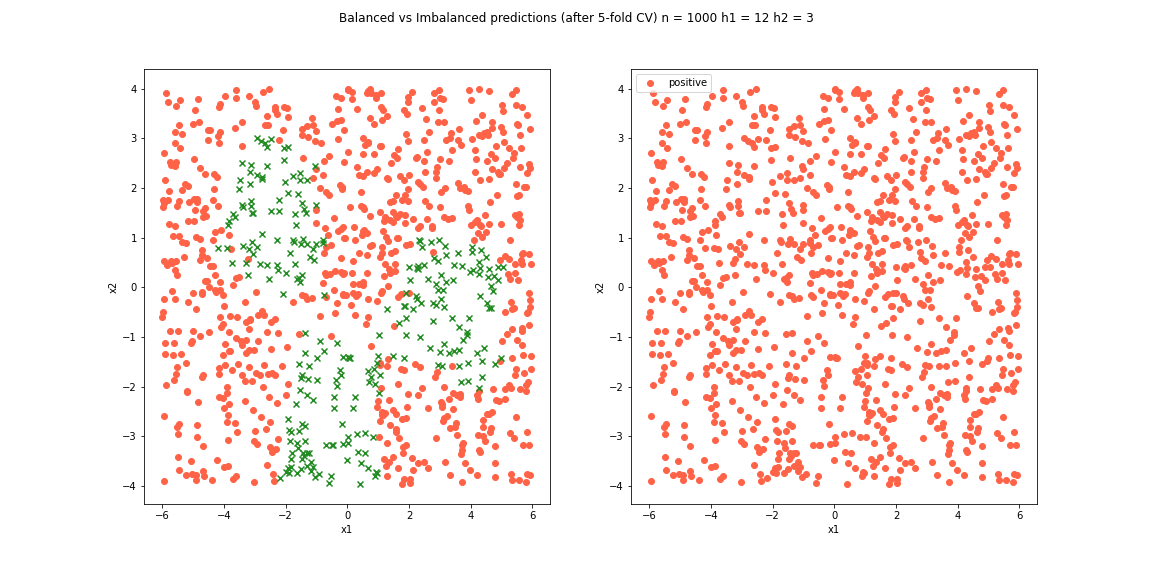
\includegraphics[width=16cm, keepaspectratio]{./3/34}
\end{figure}
\begin{figure}[H]
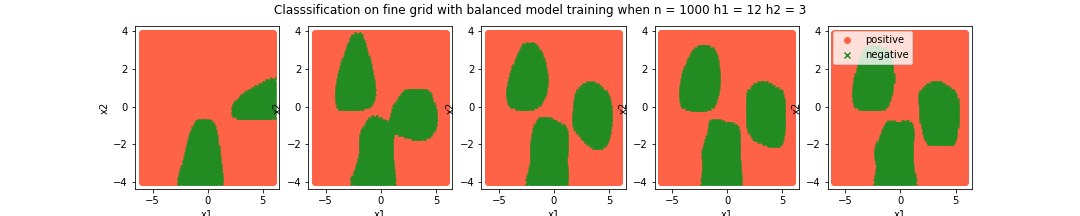
\includegraphics[width=16cm, keepaspectratio]{./3/35}
\end{figure}
\begin{figure}[H]
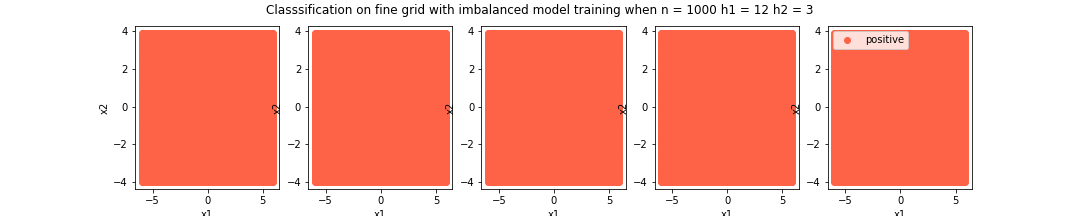
\includegraphics[width=16cm, keepaspectratio]{./3/36}
\end{figure}
\begin{figure}[H]
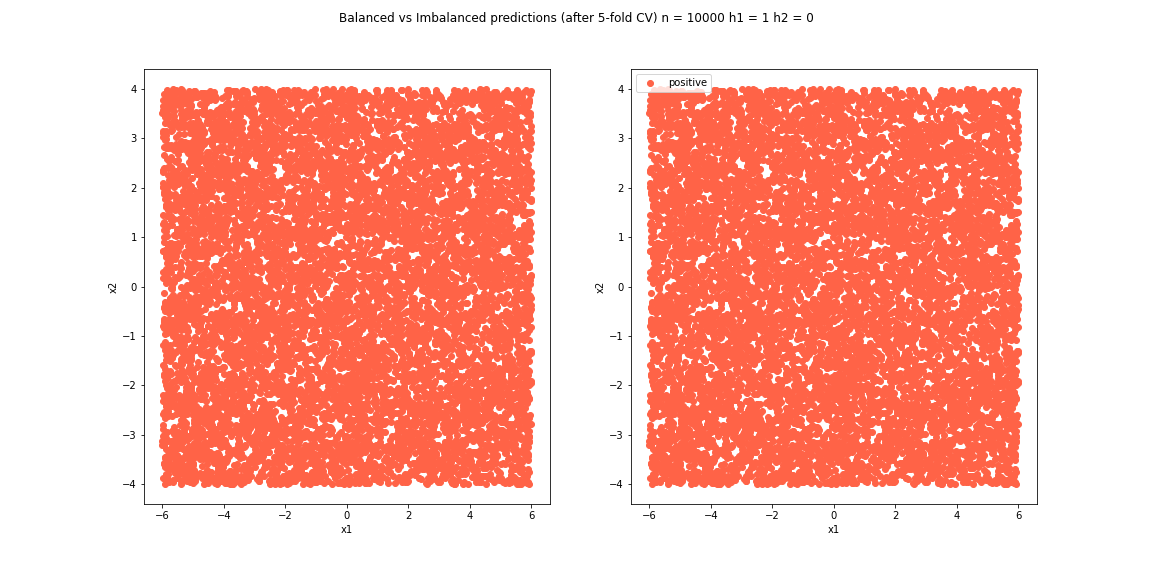
\includegraphics[width=16cm, keepaspectratio]{./3/37}
\end{figure}
\begin{figure}[H]
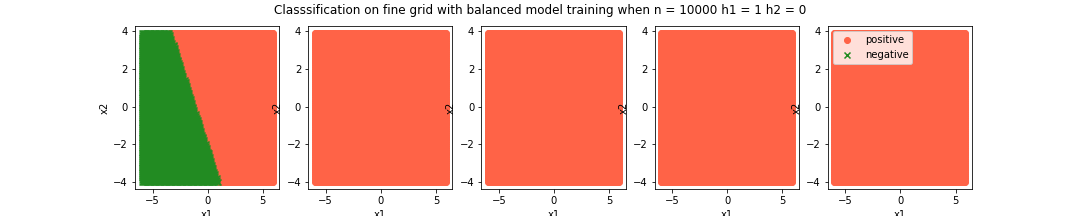
\includegraphics[width=16cm, keepaspectratio]{./3/38}
\end{figure}
\begin{figure}[H]
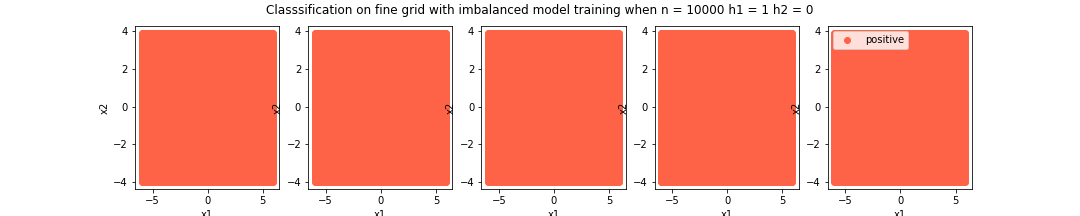
\includegraphics[width=16cm, keepaspectratio]{./3/39}
\end{figure}
\begin{figure}[H]
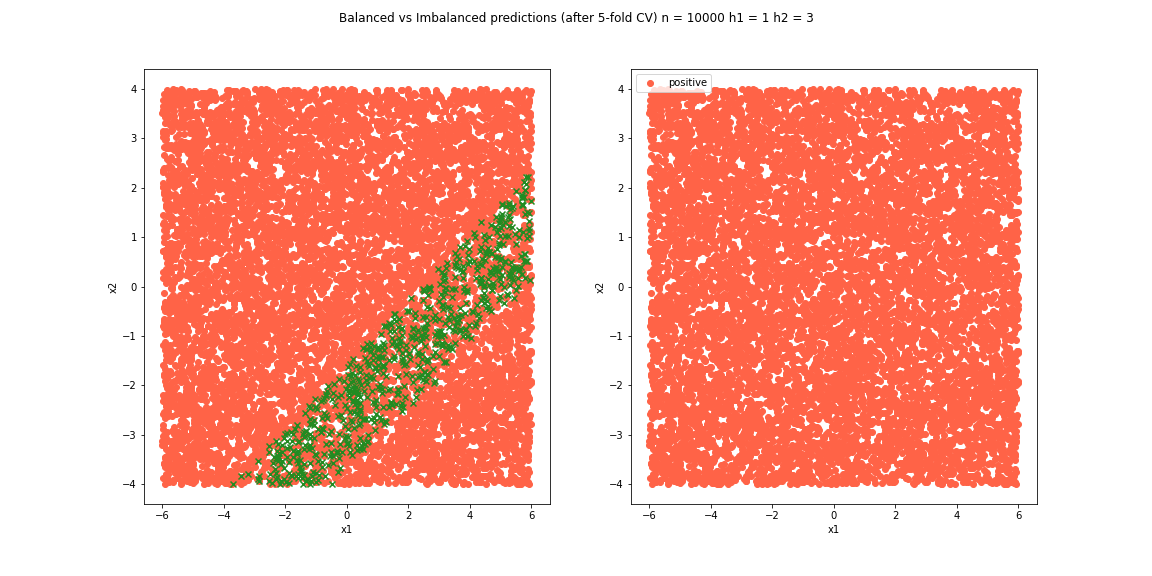
\includegraphics[width=16cm, keepaspectratio]{./3/40}
\end{figure}
\begin{figure}[H]
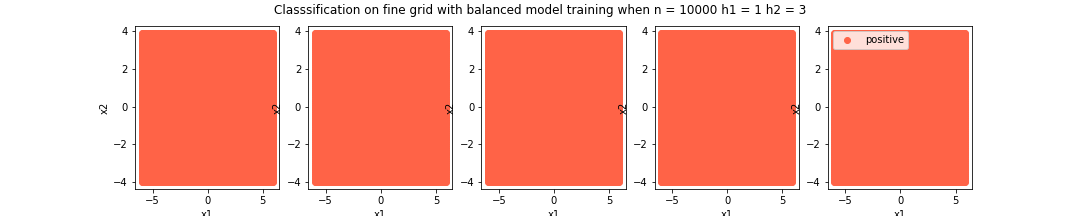
\includegraphics[width=16cm, keepaspectratio]{./3/41}
\end{figure}
\begin{figure}[H]
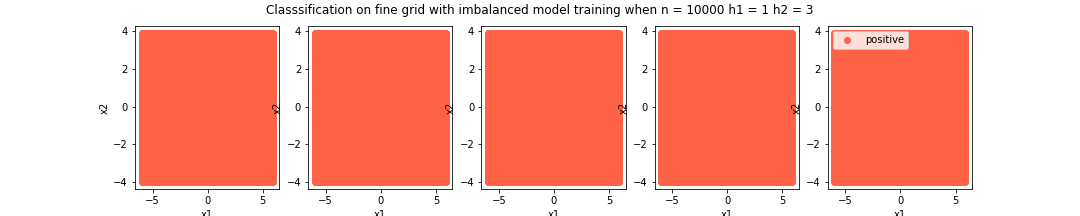
\includegraphics[width=16cm, keepaspectratio]{./3/42}
\end{figure}
\begin{figure}[H]
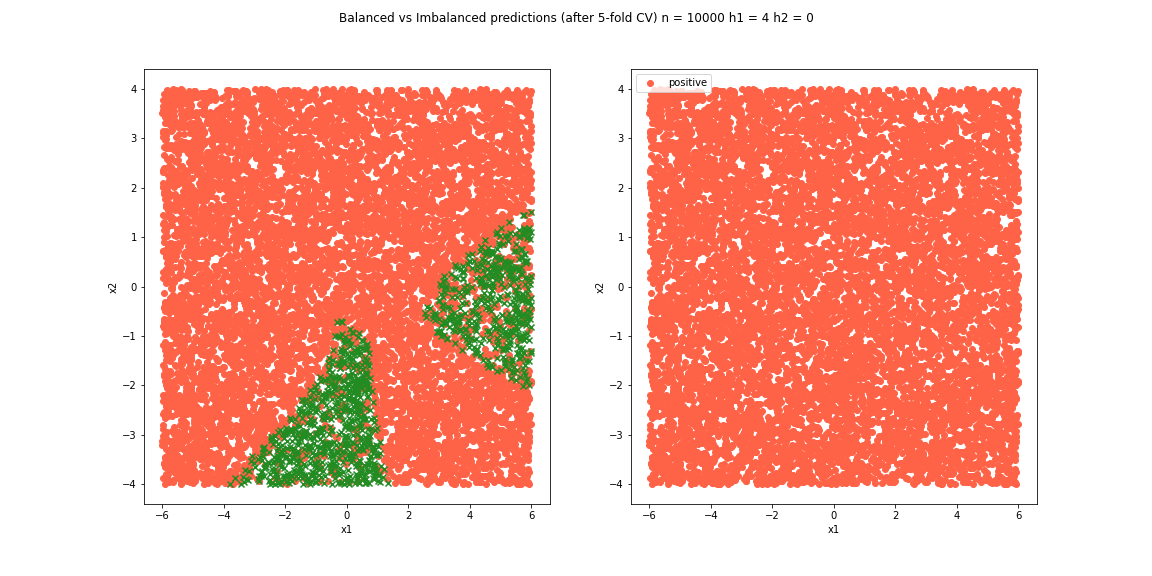
\includegraphics[width=16cm, keepaspectratio]{./3/43}
\end{figure}
\begin{figure}[H]
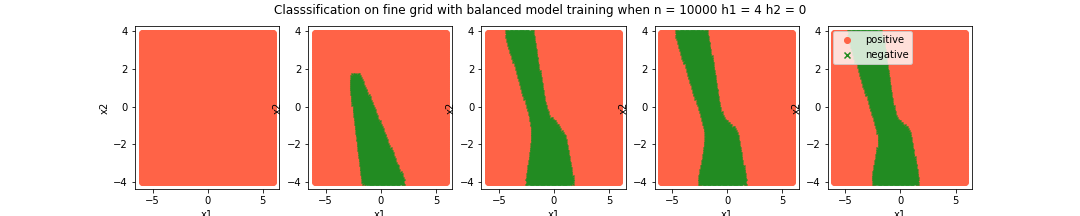
\includegraphics[width=16cm, keepaspectratio]{./3/44}
\end{figure}
\begin{figure}[H]
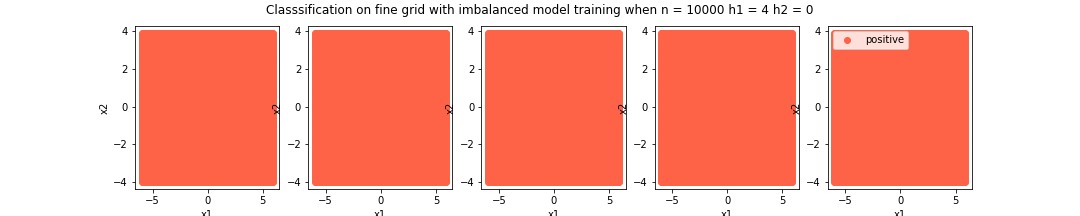
\includegraphics[width=16cm, keepaspectratio]{./3/45}
\end{figure}
\begin{figure}[H]
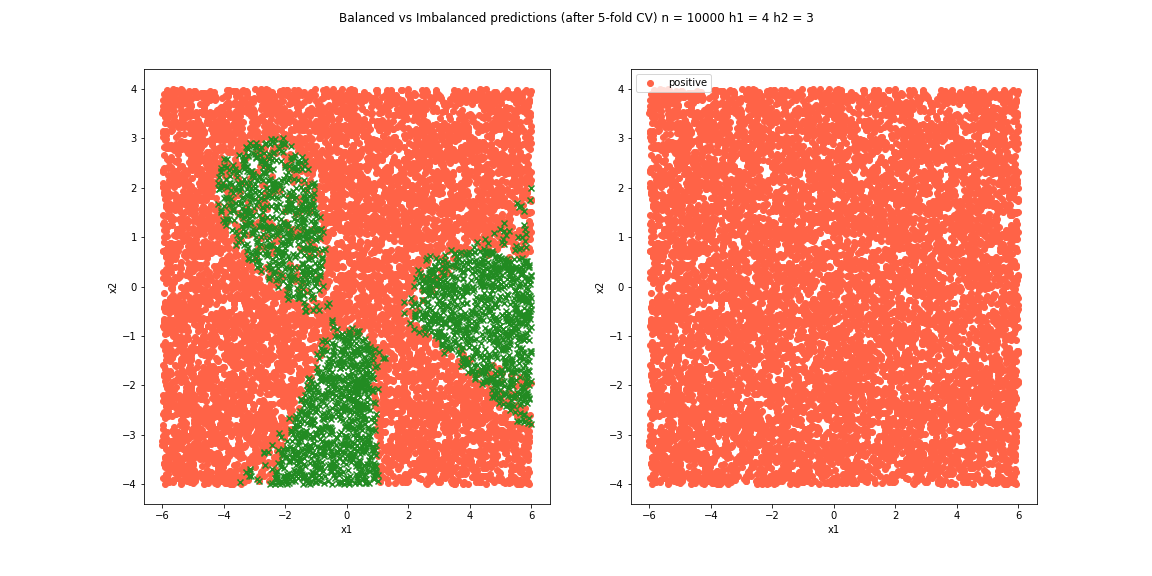
\includegraphics[width=16cm, keepaspectratio]{./3/46}
\end{figure}
\begin{figure}[H]
\includegraphics[width=16cm, keepaspectratio]{./3/47}
\end{figure}
\begin{figure}[H]
\includegraphics[width=16cm, keepaspectratio]{./3/48}
\end{figure}
\begin{figure}[H]
\includegraphics[width=16cm, keepaspectratio]{./3/49}
\end{figure}
\begin{figure}[H]
\includegraphics[width=16cm, keepaspectratio]{./3/50}
\end{figure}
\begin{figure}[H]
\includegraphics[width=16cm, keepaspectratio]{./3/51}
\end{figure}
\begin{figure}[H]
\includegraphics[width=16cm, keepaspectratio]{./3/52}
\end{figure}
\begin{figure}[H]
\includegraphics[width=16cm, keepaspectratio]{./3/53}
\end{figure}
\begin{figure}[H]
\includegraphics[width=16cm, keepaspectratio]{./3/54}
\end{figure}

\subsection*{How to read Plots}

Each of the 18 combinations of $(n, h_1, h_2)$ have 3 plots above. So, total number of plots are 54. The first plot out of the $3$ contains $2$ subplots, one containing the predictions of my network in balanced and the other contained predictions of my model in imbalanced scenarios. Each of the subplot includes outputs from all $5$ networks, $1$ each from every iteration of $5$-fold Cross Validation. The second plot contains $5$ different subplots on fine grid $1$ each for every iteration of $5$-fold Cross Validation for balanced scenario. The third plot contains $5$ different subplots on fine grid $1$ each for every iteration of $5$-fold Cross Validation for imbalanced scenario. To evaluate the performance of my performance evaluation, the plots $2$ and $3$ were drawn. The points are labeled as red dot markers for negative predictions and green cross markers for positive predictions.


\subsection*{Observations and Reasoning}

\begin{enumerate}
  \item First observation is that we can observe for the balanced scenario, Case A, for a particular $n$, the balanced accuracy, classification accuracy increases as we goes down the table. Which means the model is learning well as we increase the number of activations.
  \item Area under curve is different in almost every case because, I used soft-predictions to calculate its value. It is expected to be different because the model is trained with different configuration of activations each time. Also, it is a stochastic process and due to entropy, the value depends on the system on which the program is running. The general trend however is that it also increases as we go down the table, for a particular $n$. However there can be exceptions especially when the data is less and number of activations are less. For example, $\left(n, h_1, h_2\right) = \left(250, 1, 0\right)$ and $\left(n, h_1, h_2\right) = \left(250, 1, 3\right)$.
  \item In imbalanced class scenario (since we are choosing data from a uniform distribution), sometimes it might happen that we get points belonging to only one class as we are using $k$-fold cross validation with $k = 5$. In this case, balanced accuracy and classification accuracy would be $1.0$. However, the area under the ROC curve would be $np.nan$. When we take average of all the $k=5$ values, we still get a $np.nan$. That is why we sometimes see a $np.nan$ for area under the ROC curve in Case B. In such cases, the balanced accuracy is definitely above $0.5$ as one of the $k=5$ entries is a $1.0$.
  \item In imbalanced scenario, Case B, we can see that classification accuracy is high while the balanced accuracy is around $0.5$. Balanced accuracy is defined as the average of sensitivity (true positive rate) and specificity (true negative rate). Classification accuracy is defined as the proportion of correct predictions. This is why we should not use classification accuracy as a measure in case of imbalanced classes. We should rather prefer to use other performance metrics such as balanced accuracy or Matthews correlation coefficient. The results show that there is no learning in this case.
  \item It can be noticed from the above table that in most of the cases, it turns out that when number of activations in layer 1/layer 2 are less, the model is not learning the decision boundary properly. In case of imbalanced data, the configuration (values) of $h_1$ and $h_2$ we took in this problem is very less to learn the boundary. In case of balanced data, when the values of $h_1$ and $h_2$ are less, it doesn't learn the boundary properly. When they are relatively high $(h_1, h_2) = (12, 3)$ it is learning the boundary much better. I tried to increase the values even more $(h_1, h_2) = (100, 10)$ and it learns even better. However, in case of imbalanced classes, a configuration of $(h_1, h_2) = (1000, 20)$ also doesn't seem to learn the boundary well. This might mean that a neural network is not the right model for this problem or we can probably try adding more activations and layers.
  \item Also, the cross-validation is also 20 percent. Since the probability of getting a positive label in imbalanced data is very less it can also happen that very few positives are there in the training data (especially when $n$ is small) and the test data points are also not predicted correctly.
  \item The above conclusions are also inline with the low values for area under the ROC curve obtained in various scenarios. For example, the auc increases are we increase number of activations and decreases as the imbalance of classes increase.
  \item The results are also inline with the plots. However, results only provide the average case since were are use $k$-fold Cross Validation here with $k = 5$. If we want to know for each iteration of cross-validation, the performance of our model, plots are good tools. We can say that when number of activations are less, the learning is not so great. Still in some cases, there is learning in at least one scenario out of the $5$ iterations of cross validations. For example, the case when $\left(h_1, h_2\right) = \left(4, 0\right)$. As we increase the number of activations, the results are getting better for each iteration and the final output looks much better. Few other facts like when $\left(h_1, h_2\right) = \left(1, 0\right)$, the separation plane is sometimes like a plane because the situation here is close to (but not exactly) logistic regression.

Overall, it was a very fun exercise and I enjoyed it the most. I hope I covered almost all points. Kindly contact me if there is any discrepancy during evaluation.
\end{enumerate}




\end{solution}


\begin{problem}
Matrix factorization with applications.

a) (10 points) Derive the optimization steps for the ALS algorithm by finding formula $\# 1$ and formula $\# 2$ in the pseudocode listed above.

b) (20 points) Consider now that some values in $\mathbf{X}$ are missing (e.g., the rows of $\mathbf{X}$ are users and the columns of $\mathbf{X}$ are movie ratings, when available) and that we are interested in carrying out matrix completion using matrix factorization presented above. We would like to use the ALS algorithm, but the problem is that we must exclude all missing values from optimization. Derive now a modified ALS algorithm (formulas $\# 1$ and $\# 2$) to adapt it for matrix completion. Hint: consider adding an indicator matrix $\mathbf{W}$ to the optimization process, where $w_{ij}=1$ if $x_{ij}$ is available and $w_{ij}=0$ otherwise.

c) (20 points) Consider now a MovieLens database available at
$$
\text{http://grouplens.org/datasets/movielens/}
$$
and find a data set most appropriate to evaluate your algorithm from the previous step; e.g., one of the $100 \mathrm{k}$ data sets. Now, implement the ALS algorithm on your data set and evaluate it using the mean-squared-error as the criterion of success. You can randomly remove $25 \%$ of the ratings, train a recommendation system, and then test it on the test set. You will have to make certain decisions yourselves, such as initialization of $\mathbf{U}$ and $\mathbf{V}$, convergence criterion, or picking $k$ and $\lambda$.

d) (10 points) Describe your full experimentation process (e.g., how did you vary $k$ ) and observations from (c). Additionally, can you provide some reasoning as to what $k$ is and what matrices $\mathbf{U}$ and $\mathbf{V}$ are?

e) (10 points) Compare your method against the baseline that fills in every missing movie rating value $x_{ij}$ as an average over all users who have rated the movie $j$. Discuss your empirical findings.\end{problem}

\begin{solution}
\subsection*{a)}

Consider an $n \times d$ real-valued data matrix $\mathbf{X}=\left(\mathbf{x}_{1}^{T}, \mathbf{x}_{2}^{T}, \ldots, \mathbf{x}_{n}^{T}\right) = \left(\mathbf{x}_{1}, \mathbf{x}_{2}, \ldots, \mathbf{x}_{d}\right)$. We use the letter $i$ to denote the rows and $j$ to denote the columns. Let us approximate this matrix using the following factorization
$$
\hat{\mathbf{X}}=\mathbf{U} \mathbf{V}^{T}
$$
where $\mathbf{U}=\left(\mathbf{u}_{1}^{T}, \mathbf{u}_{2}^{T}, \ldots, \mathbf{u}_{n}^{T}\right)$ is an $n \times k$ and $\mathbf{V}=\left(\mathbf{v}_{1}^{T}, \mathbf{v}_{2}^{T}, \ldots, \mathbf{v}_{d}^{T}\right)$ is a $d \times k$ matrix of real numbers,
and where $k<n, d$ is a parameter to be explored and determined. The value $x_{ij}$ in $\mathbf{X}$ can be approximated by $\mathbf{u}_{i}^{T} \mathbf{v}_{j}$ and that $\mathbf{x}_{i}^{T},$ the $i$-th row of $\mathbf{X},$ can be approximated by $\mathbf{u}_{i}^{T} \mathbf{V}^{T},$ giving $\hat{\mathbf{x}}_{i}=\mathbf{V} \mathbf{u}_{i}$,  and $\mathbf{x}_{j},$ the $j$-th column of $\mathbf{X},$ can be approximated by $ \mathbf{U}\mathbf{v}_{j},$ giving $\hat{\mathbf{x}}_{j}=\mathbf{U} \mathbf{v}_{j}$. The matrix factorization process can be formulated as the following minimization
$$
\min _{\mathbf{U}, \mathbf{V}} \sum_{i, j}\left(x_{i j}-\mathbf{u}_{i}^{T} \mathbf{v}_{j}\right)^{2}+\lambda\left(\sum_{i}\left\|\mathbf{u}_{i}\right\|^{2}+\sum_{j}\left\|\mathbf{v}_{j}\right\|^{2}\right)
$$
which minimizes the sum-of-squared-errors between real values $x_{i j}$ and reconstructed values $\hat{x}_{i j}=\mathbf{u}_{i}^{T} \mathbf{v}_{j}$. The regularization parameter $\lambda \geq 0$ is user-selected. This problem can be directly solved using gradient descent, but we will attempt a slightly different approach. To do this, we can see that for a fixed $\mathbf{V}$ we can find optimal vectors $\mathbf{u}_{i}$ by minimizing,
$$
L_{1} = \left\|\mathbf{V} \mathbf{u}_{i}-\mathbf{x}_{i}\right\|^{2}+\lambda \cdot\left\|\mathbf{u}_{i}\right\|^{2}
$$
which can be solved in a closed form using OLS regression for every $i$. Taking the derivative and equating to $0$, we get,


\begin{align*}
	\pdv{L_1}{\mathbf{u}_i} &= \pdv{}{\mathbf{u}_i}\left(\mathbf{u}_i^{T}\mathbf{V}^{T}\mathbf{V}\mathbf{u}_i - \mathbf{u}_i^{T}\mathbf{V}^{T}\mathbf{x}_{i} - \mathbf{x}_{i}^{T}\mathbf{V}\mathbf{u}_i + \mathbf{x}_{i}^{T}\mathbf{x}_{i} + \lambda\mathbf{u}_i^{T}\mathbf{u}_i\right)\\
	&= 2\mathbf{V}^{T}\mathbf{V}\mathbf{u}_i - \mathbf{V}^{T}\mathbf{x}_i - \mathbf{V}^{T}\mathbf{x}_i + 0 + 2\lambda\mathbf{u}_i\\
	&= 2\left(\left(\mathbf{V}^{T}\mathbf{V}+\lambda\mathbf{I}\right)\mathbf{u}_i - \mathbf{V}^{T}\mathbf{x}_i\right)\\
	&= 0\\
\end{align*}
$$
	\implies \boxed{\mathbf{u}_i = \left(\mathbf{V}^{T}\mathbf{V}+\lambda\mathbf{I}\right)^{-1}\mathbf{V}^{T}\mathbf{x}_i}
$$

We can equivalently express the optimization for vectors $\mathbf{v}_{j}$ and find the solution for every $j$. It will be like minimizing,
$$
L_{2} = \left\|\mathbf{U} \mathbf{v}_{j}-\mathbf{x}_{j}\right\|^{2}+\lambda \cdot\left\|\mathbf{v}_{j}\right\|^{2}
$$
which can be solved in a closed form using OLS regression for every $j$. Please note that $\mathbf{x}_j$ here is the column vector of matrix $\mathbf{X}$. Taking the derivative and equating to $0$, we get,

\begin{align*}
	\pdv{L_2}{\mathbf{v}_j} &= \pdv{}{\mathbf{v}_j}\left(\mathbf{v}_j^{T}\mathbf{U}^{T}\mathbf{U}\mathbf{v}_j - \mathbf{v}_j^{T}\mathbf{U}^{T}\mathbf{x}_{j} - \mathbf{x}_{j}^{T}\mathbf{U}\mathbf{v}_j + \mathbf{x}_{j}^{T}\mathbf{x}_{j} + \lambda\mathbf{v}_j^{T}\mathbf{v}_j\right)\\
	&= 2\mathbf{U}^{T}\mathbf{U}\mathbf{v}_j - \mathbf{U}^{T}\mathbf{x}_j - \mathbf{U}^{T}\mathbf{x}_j + 0 + 2\lambda\mathbf{v}_j\\
	&= 2\left(\left(\mathbf{U}^{T}\mathbf{U}+\lambda\mathbf{I}\right)\mathbf{v}_j - \mathbf{U}^{T}\mathbf{x}_j\right)\\
	&= 0\\
\end{align*}
$$
	\implies \boxed{\mathbf{v}_j = \left(\mathbf{U}^{T}\mathbf{U}+\lambda\mathbf{I}\right)^{-1}\mathbf{U}^{T}\mathbf{x}_j}
$$

\subsection*{b)}

I am using the same notations as used in part a) (for ex: $i$ denotes rows and $j$ denotes columns). Let some values in $\mathbf{X}$ are missing. Consider an indicator matrix $\mathbf{W}$ to the optimization process, where $w_{ij}=1$ if $x_{ij}$ is available and $w_{ij}=0$ otherwise. The matrix factorization process can be modified and formulated as the following minimization,
$$
\min _{\mathbf{U}, \mathbf{V}} \mathbf{W} \odot \left\|\mathbf{X}-\mathbf{U} \mathbf{V}^{T}\right\|^{2}+\lambda\left(\left\|\mathbf{U}\right\|^{2}+\left\|\mathbf{V}\right\|^{2}\right)
$$
$$\text{(or)}$$
$$
\min _{\mathbf{U}, \mathbf{V}} \left\|\sqrt{\mathbf{W}} \odot \left(\mathbf{X}-\mathbf{U} \mathbf{V}^{T}\right)\right\|^{2}+\lambda\left(\left\|\mathbf{U}\right\|^{2}+\left\|\mathbf{V}\right\|^{2}\right)
$$
$$\text{(or)}$$
$$
\min _{\mathbf{U}, \mathbf{V}} \sum_{i, j}w_{ij}\left(x_{i j}-\mathbf{u}_{i}^{T} \mathbf{v}_{j}\right)^{2}+\lambda\left(\sum_{i}\left\|\mathbf{u}_{i}\right\|^{2}+\sum_{j}\left\|\mathbf{v}_{j}\right\|^{2}\right)
$$

where $\odot$ means the Hadamard product (element-wise product).

The above objective function minimizes the sum-of-squared-errors between real non-missing values $x_{ij}$ and reconstructed values $\hat{x}_{i j}=\mathbf{u}_{i}^{T} \mathbf{v}_{j}$. The regularization parameter $\lambda \geq 0$ is user-selected. This problem can be directly solved using gradient descent, but we will attempt a slightly different approach. To do this, we can see that for a fixed $\mathbf{V}$ we can find optimal vectors $\mathbf{u}_{i}$ by minimizing,
\begin{align*}
L_{1} &= \left\|\sqrt{\mathbf{W}^{i}}\left(\mathbf{V} \mathbf{u}_{i}-\mathbf{x}_{i}\right)\right\|^{2}+\lambda \cdot\left\|\mathbf{u}_{i}\right\|^{2}\\
      &= \left(\mathbf{V}\mathbf{u}_i-\mathbf{x}_i\right)^{T}\mathbf{W}^{i}\left(\mathbf{V}\mathbf{u}_i-\mathbf{x}_i\right) + \lambda\mathbf{u}_i^{T}\mathbf{u}_i
\end{align*}
where, $\mathbf{W}^{i}$ is a diagonal matrix whose elements in diagonal are the elements of $i^{\text{th}}$ row of matrix $\mathbf{W}$, i.e., $\mathbf{W}^{i} = \text{diag}\left(w_{i1}, w_{i2}, ..., w_{id}\right)$.

This problem can be solved in a closed form using OLS regression for every $i$. Taking the derivative and equating to $0$, we get,


\begin{align*}
	\pdv{L_1}{\mathbf{u}_i} &= \pdv{}{\mathbf{u}_i}\left(\left(\mathbf{V}\mathbf{u}_i-\mathbf{x}_i\right)^{T}\mathbf{W}^{i}\left(\mathbf{V}\mathbf{u}_i-\mathbf{x}_i\right) + \lambda\mathbf{u}_i^{T}\mathbf{u}_i\right)\\
	&= -2\mathbf{V}^{T}\mathbf{W}^{i}\left(\mathbf{x}_i-\mathbf{V}\mathbf{u}_i\right) + 2\lambda\mathbf{u}_i\\
	&= 2\left(-\mathbf{V}^{T}\mathbf{W}^{i}\mathbf{x}_i+\mathbf{V}^{T}\mathbf{W}^{i}\mathbf{V}\mathbf{u}_i+\lambda\mathbf{u}_i\right)\\
	&= 0\\
\end{align*}
$$
	\implies \boxed{\mathbf{u}_i = \left(\mathbf{V}^{T}\mathbf{W}^{i}\mathbf{V}+\lambda\mathbf{I}\right)^{-1}\mathbf{V}^{T}\mathbf{W}^{i}\mathbf{x}_i}
$$

We can equivalently express the optimization for vectors $\mathbf{v}_{j}$ and find the solution for every $j$. It will be like minimizing,
\begin{align*}
L_{2} &= \left\|\sqrt{\mathbf{W}^{j}}\left(\mathbf{U} \mathbf{v}_{j}-\mathbf{x}_{j}\right)\right\|^{2}+\lambda \cdot\left\|\mathbf{v}_{j}\right\|^{2}\\
      &= \left(\mathbf{U}\mathbf{v}_j-\mathbf{x}_j\right)^{T}\mathbf{W}^{j}\left(\mathbf{U}\mathbf{v}_j-\mathbf{x}_j\right) + \lambda\mathbf{v}_j^{T}\mathbf{v}_j
\end{align*}

where, $\mathbf{W}^{j}$ is a diagonal matrix whose elements in diagonal are the elements of $j^{\text{th}}$ column of matrix $\mathbf{W}$, i.e., $\mathbf{W}^{j} = \text{diag}\left(w_{1j}, w_{2j}, ..., w_{nj}\right)$.

This problem can be solved in a closed form using OLS regression for every $j$. Please note that $\mathbf{x}_j$ here is the column vector of matrix $\mathbf{X}$. Taking the derivative and equating to $0$, we get,

\begin{align*}
	\pdv{L_2}{\mathbf{v}_j} &= \pdv{}{\mathbf{v}_j}\left(\left(\mathbf{U}\mathbf{v}_j-\mathbf{x}_j\right)^{T}\mathbf{W}^{j}\left(\mathbf{U}\mathbf{v}_j-\mathbf{x}_j\right) + \lambda\mathbf{v}_j^{T}\mathbf{v}_j\right)\\
	&= -2\mathbf{U}^{T}\mathbf{W}^{j}\left(\mathbf{x}_j-\mathbf{U}\mathbf{v}_j\right) + 2\lambda\mathbf{v}_j\\
	&= 2\left(-\mathbf{U}^{T}\mathbf{W}^{j}\mathbf{x}_j+\mathbf{U}^{T}\mathbf{W}^{j}\mathbf{U}\mathbf{v}_j+\lambda\mathbf{v}_j\right)\\
	&= 0\\
\end{align*}
$$
	\implies \boxed{\mathbf{v}_j = \left(\mathbf{U}^{T}\mathbf{W}^{j}\mathbf{U}+\lambda\mathbf{I}\right)^{-1}\mathbf{U}^{T}\mathbf{W}^{j}\mathbf{x}_j}
$$

\subsection*{c) \&  d)}

For code, please refer to \textbf{MatrixFactorization.ipynb}.

I chose the \texttt{ml-100k} dataset\cite{movielens100} from MovieLens. This data set consists of:
\begin{itemize}
	\item 100,000 ratings (1-5) from 943 users on 1,682 movies. 
	\item Each user has rated at least 20 movies. 
	\item Simple demographic info for the users (age, gender, occupation, zip)
\end{itemize}

The data was collected through the MovieLens web site (movielens.umn.edu) during the seven-month period from September 19th, 1997 through April 22nd, 1998. This data has been cleaned up - users who had less than 20 ratings or did not have complete demographic information were removed from this data set. Detailed descriptions of the data file can be found at the end of this file.

The dataset \texttt{ml-100/u.data} contains $4$ columns, namely, \texttt{user\_id}, \texttt{movie\_id}, \texttt{rating} and \texttt{timestamp}. There are totally $100,000$ entries in this data. There are a total of $n = 943$ users and $d = 1,682$ movies. Since, $100000 \ne 943 \times 1682$, we must be having missing values in matrix $\textbf{X}$ with $n$ rows and $d$ columns. Our goal is to represent this matrix as product of $\textbf{U}$ and $\textbf{V}^{T}$ as per the objective function mentioned in parts a) and b). In order to take care of missing values, an indicator matrix $\textbf{W}$ is formed such that $w_{ij} = 0$ if $x_{ij}$ is missing, else $w_{ij} = 1$. Since, the input is highly sparse, I am unable to extract an exact $25 \%$ of the set to use it as testing data. If I try to extract $25 \%$ randomly, there is a chance that there can be columns with all zeroes in the training data and this implies that the training may not be so effective. Hence, I chose $100$ columns for every user from the training set where the input is dense (i.e., from a set of top $1000$ values where there are so many user ratings for the movies). If this is not working for some reason in your computer, please try re-running or reducing the value $100$. This strategy had been doubled checked with Professor during office hours and got a confirmation that this is a valid strategy. So, I have training and test data matrices of same size as input $n \times k$, but training data matrix contains $100n$ extra missing values shifted to test data matrix as per the logic mentioned above. I also made sure that training and test dataset are disjoint. Indirectly, the split is also a hyperparameter (although not a standard one). Feel free to try different values. The implementation of ALS is fairly straightforward as it is finding the vectors $\textbf{u}_i$ and $\textbf{v}_j$ as shown above.

The most important hyperparameter in the entire exercise is $k$. I varied $k$ according to the values in the list \texttt{k\_list = [5, 10, 20, 40, 80]}. $k$ represents the so called \textbf{Concepts} or \textbf{Latent Factors}. If there is knowledge the data is coming from $k$ categories, we can simply use that domain knowledge and achieve great performances. In this example of movies and ratings, $k$ can be thought of as \textbf{genres} of the movies. This hyperparameter is similar to the hyperparameter $y$ in \textbf{EM-Algorithm}. Even there if we have prior knowledge about the data that is comes from $y$ distributions, we can calculate the parameters of the actual distributions effectively. Because of this presence of latent variable, the \textbf{MatrixFactorization} can be thought of as an unsupervised learning problem. It is well known in the industry as \textbf{Collaborative Filtering}. In this problem, I have considered that the weights to be uniform (either $0$ or $1$ depending on values are missing or available). Further reasearch is actively going on on this and we can even have non-uniform weights\cite{nonuniform_mf} to obtain a beter low rank matrix factorization for real world problems.

The initialization of matrices \textbf{U} and \textbf{V} are done randomly using the function \texttt{numpy.random.random\_sample} which return values from the 'continuous uniform' distribution over the interval \texttt{[0.0, 1.0)}. The final output matrix

\begin{enumerate}
	\item $\mathbf{U} \in \mathbb{R}^{n \times k}$ is a user embedding matrix, where row $i$ is the embedding for user $i$.
	\item $\mathbf{V} \in \mathbb{R}^{d \times k}$ is an item embedding (in this case items are movies) matrix, where row $j$ is the embedding for item (movie) $j$.
\end{enumerate}

One more hyperparameter involved is regularization constant $\lambda$. It is a value chosen from the list \texttt{lmd\_list = [0.1, 2, 5, 10, 25, 50, 100]} once per iteration. Number of iterations (epochs) is another hyperparamter. It is a value chosen from the list \texttt{epochs\_list = [1, 2, 5, 10]} once per iteration and trained incrementally to avoid over-training. Refer to my code for a better understanding.

The evaluation of the predictions is done using $mean\_square\_error$, which considers only non-zero/non-missing values from the input.

After this entire experiment, the best combination of hyperparamters (with the corresponding train and test errors) obtained for my experiment are as follows:

\begin{lstlisting}[language=Python]
{'epochs': 10,
 'k': 5,
 'lambda': 5,
 'train_error': 0.6672904167634547,
 'test_error': 0.8236433053485411}
\end{lstlisting}


The whole experiment takes approximately $15$ minutes to run and get results. I highly recommend using Google Colab (setup below) in order to verify the results:

\texttt{https://colab.research.google.com/drive/1u8FoCOaL9ugfm8udb7MYYgFeOyLQPObW?usp=sharing}\\

A random seed is already set to $42$ in order to replicate the results. Make sure to change path to file in Data Cell numbered [2].\\

\subsection*{e)}

In order to see how the model performs as compared to mean, I have taken the train dataset and fill those $100n$ values transferred to test data with the mean of rest of the non zero values in the column. This strategy has been quadruple checked with Professor in office hours. Once, the mean is imputed in those removed cells of training data, I call the $get\_mse$ method and calculate the mean square error using those $100n$ values where the cells in test data has non-zero ratings. This is done to see how our model performs when compared to mean prediction. Here are the results:

\begin{lstlisting}[language=Python]
{'k': 5,
 'lambda': 5,
 'epochs': 10,
 'train_error': 0.6672904167634547,
 'test_error': 0.8236433053485411,
 'mean_error': 0.3025307958188201}
\end{lstlisting}

From the above results, it can be noticed that for $k = 5$ and $\lambda = 5$ with $10$ epochs, we get train\_error as $0.667$, test\_error as $0.824$ and $mean\_error$ as $0.303$. The train\_error and test\_error are relatively comparable and also quite less ($< 1$) in magnitude. This means that our model is robust. However, when compared to test\_error, mean\_error is quite less. Although there is a chance that our model is performing poorly compared to the basic mean prediction, I think this is a misleading conclusion because our observations is based out of training $943 \times 1582$ data points and validating against $943 \times 100$ data points. This is relatively sort of over-fitting and I see there is a chance of high variance involved in my experiment. However, I was unable to avoid it, as I want to select records such that I have at least some non zero ratings for every movie in the training data. The model however, turned out to be robust. I am anyway left with only $943 \times 100$ records in order to compute mean square error and compare mean prediction with my model predictions. If we have more testing data, it might most likely turn out that I will get a high mean\_error. Or the vice versa can also happen if my model has high variance which is unlikely as the difference between train error and test error is very less. However, one more important point to note is that, it makes more sense to think that mean predictions are not bad in this problem of user-movie rating because if $p$ persons are liking/disliking a particular movie, it is most likely that $p + 1^{th}$ also likes/dislikes it. The distribution of mean ratings for different samples of a paricular movie can be assumed to approximately follow a normal distribution with low variance and almost tending to a dirac delta spike according to weak law of large numbers\cite{lln}.


\end{solution}


\begin{problem}
Prove representational equivalence of a three-layer neural network with linear activation function in all neurons and a single-layer layer neural network with the same activation function. Assume a single-output network.
\end{problem}

\begin{solution}
\begin{figure}[H]
\includegraphics[width=16cm, keepaspectratio]{NeuralNetwork}
\caption{A three-layer neural network}
\end{figure}

The above neural network, consists of $1$ input layer, $2$ hidden layers and $1$ output layer. Here, $a^{[i]}$ represents the vector of activations present in the $i^{\text{th}}$ layer, $w^{[i]}$ represents the vector of weights for activations present in the $i^{\text{th}}$ layer. $X$ is the input feature vector of $d$-dimensions. Hidden layer 1 contains $d_1$-activations and a bias, hidden layer 2 contains $d_2$-activations and a bias. $\hat{y}$ represents the output. $a^{[i]}_{j}$ represents $j^{\text{th}}$ activation in the $i^{\text{th}}$ layer. $w^{[i]}_{jk}$ represents the weight connection $j^{\text{th}}$ activation present in $i^{\text{th}}$ layer to the $k^{\text{th}}$ activation present in the $i-1^{\text{th}}$ layer. $x_i$ represents the $i^{\text{th}}$ input data point.

Let, $d_0 = d$ for notation simplification. Let us consider a linear activation function $h(z) = c_1z +c_2$.

Applying the activation function to the activations, we can construct $d_{l-1}$ linear combinations of activations in $l-1^{\text{th}}$ layer, after which the $j_{\text{th}}$ activation in the $l^{\text{th}}$ layer would look like,
\begin{align*}
a^{[l]}_{j} &= \sum_{i = 1}^{d_{l-1}} w^{[l]}_{ji}h\left(a^{[l-1]}_{i}\right) + w^{[l]}_{j0}\\
			  &= \sum_{i = 1}^{d_{l-1}} w^{[l]}_{ji}\left(c_1a^{[l-1]}_{i}+c_2\right) + w^{[l]}_{j0}\\
			  &= \sum_{i = 1}^{d_{l-1}} c_1w^{[l]}_{ji}a^{[l-1]}_{i}+\sum_{i = 1}^{d_{l-1}}c_2 w^{[l]}_{ji} + w^{[l]}_{j0}\\
			  &= \sum_{i = 1}^{d_{l-1}} {w^{'}}^{[l]}_{ji}a^{[l-1]}_{i} + {w^{'}}^{[l]}_{j0}\\
			  &= \sum_{i = 0}^{d_{l-1}} {w^{'}}^{[l]}_{ji}a^{[l-1]}_{i}
\end{align*}

where in the above equations constants are absorbed and the weights of the new terms are represented by $w{'}$ that are linear tranformations of the original ones.

Let's try to represent activations of layer $l$ in terms of $l - 2$.
\begin{align*}
a^{[l]}_{j} &= \sum_{i = 0}^{d_{l-1}} {w^{'}}^{[l]}_{ji}a^{[l-1]}_{i}\\
			  &= \sum_{i = 0}^{d_{l-1}} {w^{'}}^{[l]}_{ji}\left(\sum_{k = 0}^{d_{l-2}} {w^{'}}^{[l-1]}_{jk}a^{[l-2]}_{k}\right)\\
			  &= \sum_{k = 0}^{d_{l-2}} {w^{''}}^{[l-1]}_{jk}a^{[l-2]}_{k}
\end{align*}

where in the above equations constants are absorbed and the weights of the new terms are represented by $w{''}$ that are linear tranformations of the ones obtained in the previous steps.

Since, the above tranformation is linear (similar to Linear Regression), we can skip hidden layer 1 and go to hidden layer 2, with similar weights and skip layer 2 and go to layer 3 (output layer) with similar weights. The final representation of the neural network from layer 0 (input layer) to layer 3 (output layer) can be represented as,

$$
a^{[3]}_{j} = \sum_{i = 0}^{d_0} {w^{'''}}^{[0]}_{ji}a^{[0]}_{i}
$$

or

\begin{equation}
\hat{y} = \sum_{i = 0}^{d} {w^{'''}}^{[0]}_{ji}x_{i}
\end{equation}

If we have a $1$-layered neural network with $1$-output and linear activation function, this can be thought similar to Linear Regression, whose general form is,

\begin{equation}
\hat{y} = \sum_{i = 0}^{d} {w}^{[0]}_{ji}x_{i}
\end{equation}

Equations $(1)$ and $(2)$ are representationally equivalent. Hence, proved.

\end{solution}



\begin{problem}
Let $A, B, C,$ and $D$ be binary input variables (features). Give decision trees to represent the following Boolean functions:

a) $(3$ points $) A \wedge \bar{B}$

b) $(3$ points $) A \vee(\bar{B} \wedge C)$

c) $(4$ points $) A \oplus \bar{B}$\\
where $\bar{A}$ is the negation of $A$ and $\oplus$ is an exclusive OR operation.
\end{problem}

\begin{solution}
We can replace 'T' with $1$ and 'F' with $0$ and still obtain the same outputs in the end.
\begin{figure}[H]
\includegraphics[width=5.5cm, keepaspectratio]{Problem6_a}
\caption{a) $A \wedge \bar{B}$}
\end{figure}
\begin{figure}[H]
\includegraphics[width=5.5cm, keepaspectratio]{Problem6_b}
\caption{b) $A \vee(\bar{B} \wedge C)$}
\end{figure}
\begin{figure}[H]
\includegraphics[width=5.5cm, keepaspectratio]{Problem6_c}
\caption{c) $A \oplus \bar{B}$}
\end{figure}


\end{solution}


\medskip

\begin{thebibliography}{9}
\bibitem{movielens100}
F. Maxwell Harper and Joseph A. Konstan. 2015. \textit{The MovieLens Datasets: History and Context. ACM Transactions on Interactive Intelligent Systems (TiiS) 5, 4, Article 19 (December 2015), 19 pages.}
\\\texttt{DOI=http://dx.doi.org/10.1145/2827872}

\bibitem{nonuniform_mf}
Xiangnan He, Jinhui Tang, Senior Member, IEEE, Xiaoyu Du, Richang Hong, Member, IEEE, Tongwei Ren, Member, IEEE, and Tat-Seng Chua. 2018. \textit{Fast Matrix Factorization with Non-Uniform Weights on Missing Data}
\\\texttt{DOI=https://arxiv.org/pdf/1811.04411.pdf}

\bibitem{lln}
Routledge, R. (2016, October 12). \textit{Law of large numbers. Encyclopedia Britannica.}
\\\texttt{URL: https://www.britannica.com/science/law-of-large-numbers}
\end{thebibliography}


\end{document}

\end{document}